%-------------------------------------------------------------------------------
\section{Einführung in die Vorlesung}
%-------------------------------------------------------------------------------

%%% Folie
\begin{frame}{Vorstellung: Martin Kutscher}
    \begin{columns}
        \begin{column}{.2\textwidth}
            \begin{center}
                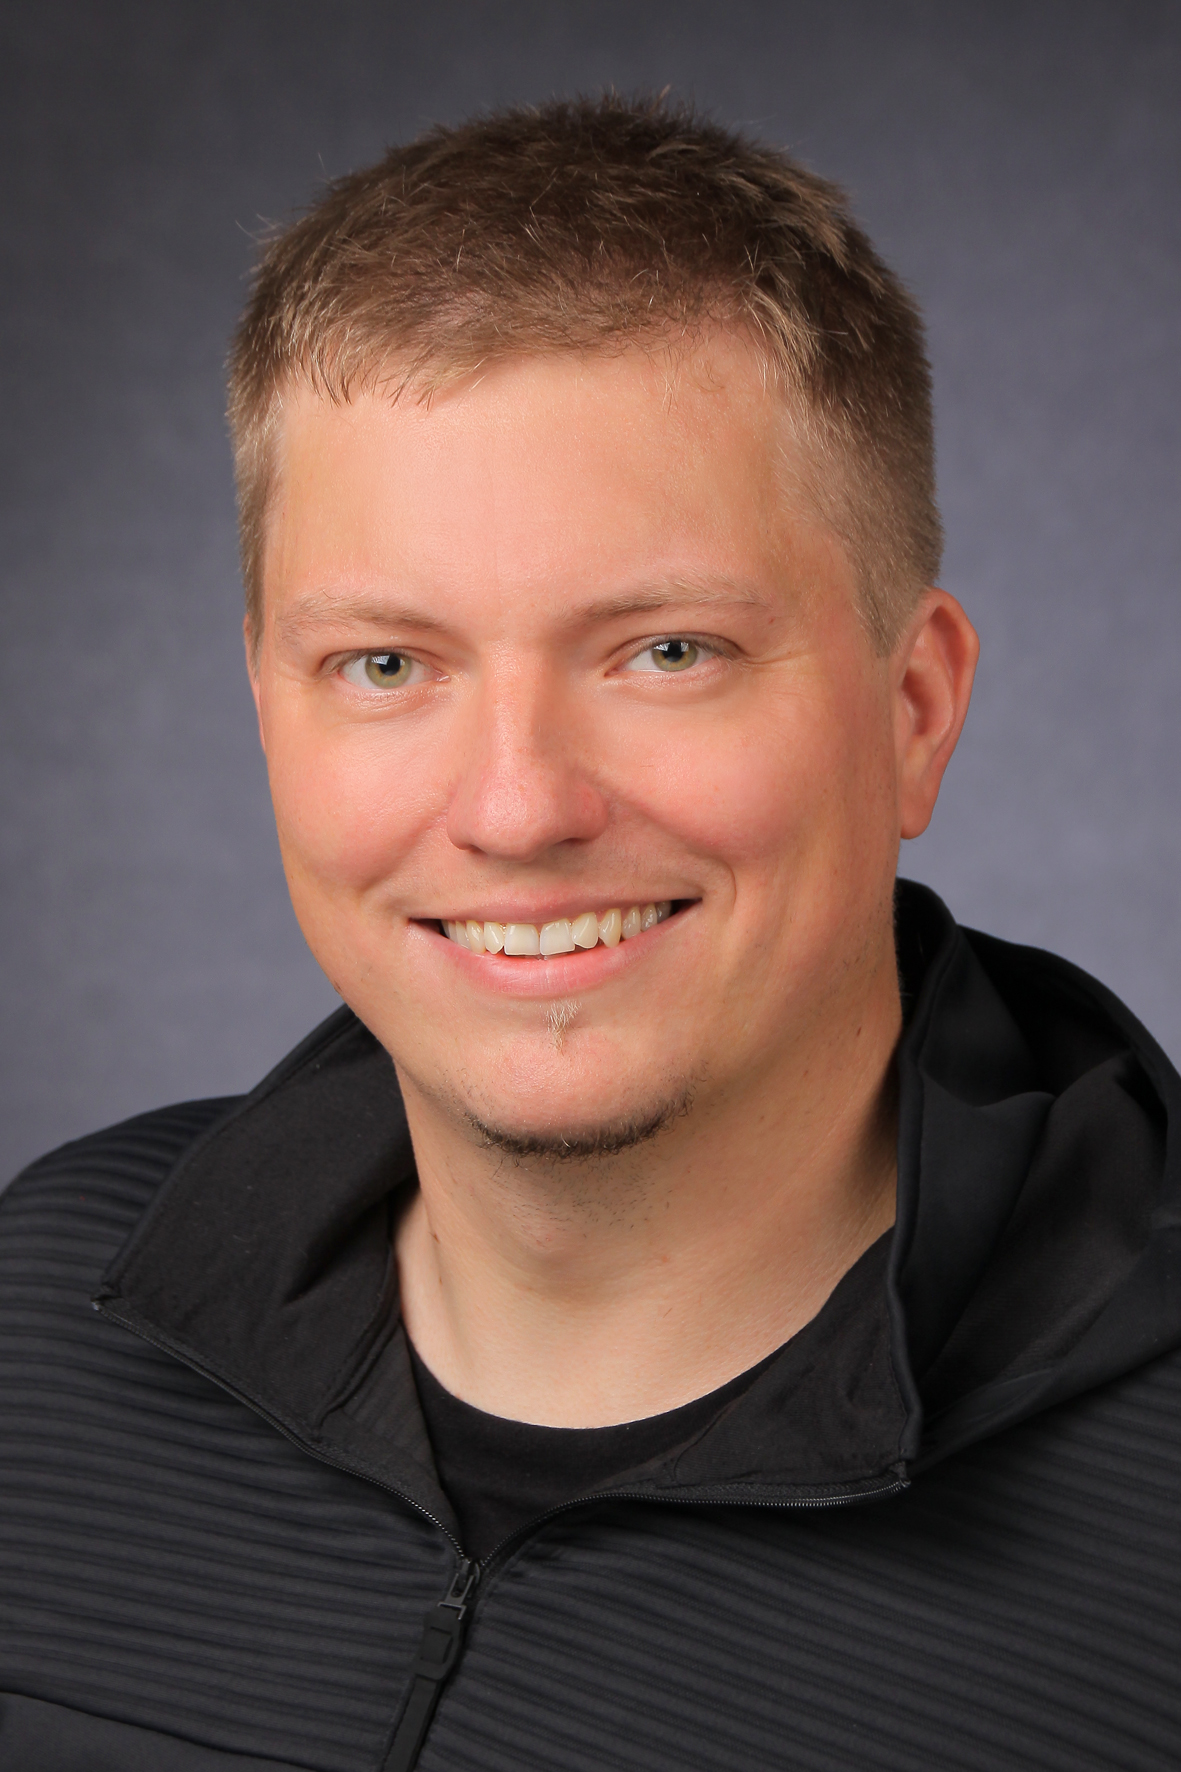
\includegraphics[width=\textwidth]{1-grundlagen/img/dozent_kutscher}
            \end{center}
        \end{column}
        \begin{column}{.8\textwidth}
            \begin{itemize}
                \item \textbf{2012:} Diplom ,,Angewandte Informatik''  an der Uni Duisburg-Essen
                mit Vertiefung ,,Verteilte Systeme und Embedded Systems''

                \item \textbf{2011 -- 2012:} Android-Entwicklung im SKIMS Projekt
                (\Href{https://skims.realmv6.org/})

                \item \textbf{2012 -- aktuell:} IT-Consultant bei EXXETA, Schwerpunkte vor allem
                Web-Entwicklung (Full Stack Development), JavaEE Backend, Angular sowie Integration
                von Backendsystemen wie SAP etc.

                \item \textbf{2016 -- aktuell:} IoT-Projekt SMIGHT (\Href{https://demo.smight-mgt.de}),
                Entwicklung von Microservices mit Node.js und SpringBoot in TypeScript, Java und
                Kotlin, Java OSGI Clients für den Raspberry PI

                \item \textbf{Seit 2018:} Dozent an der DHBW Karlsruhe für
                IoT-Integrationsseminar und Projekt, Verteilte Systeme, Hardwarenahe Programmierung
            \end{itemize}
        \end{column}
    \end{columns}
\end{frame}

%%% Folie
\begin{frame}{Vorstellung: Dennis Schulmeister-Zimolong}
    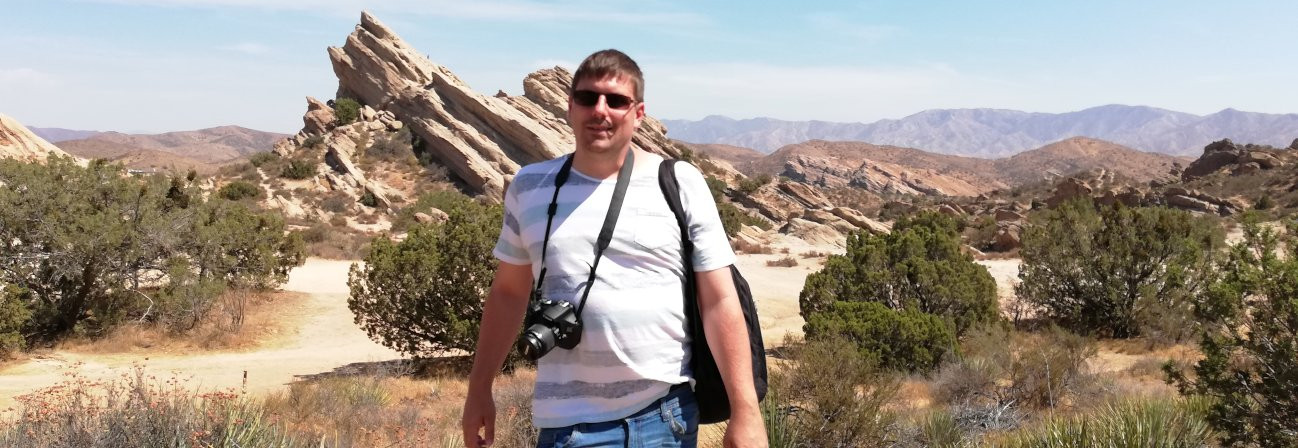
\includegraphics[width=\textwidth]{1-grundlagen/img/dozent_schulmeister}

    \begin{itemize}
        \item Dipl.-Wirtschaftsinformatiker (DH), DHBW Karlsruhe, 2005 – 2008
        \item Produktmanager / Senior Entwickler für SAP Add-Ons, cormeta ag
        \item Seit 2009 nebenberuflicher Dozent an der DHBW Karlsruhe
        \item Seit 1992 begeistert von Computern und deren Programmierung
        \item Keyboarder, Bassist, Sänger und Songwriter in der Freizeit
        \item Seit 2018 am verzweifeln am Golfschwung \smiley{}
    \end{itemize}
\end{frame}

%%% Folie
\begin{frame}{Kompetenzziele dieser Vorlesung}
    \begin{itemize}[<+->]
        \item \textbf{Fachkompetenz:} Die Studierenden kennen den technischen Aufbau typischer
        Devices/Embedded Systems im Kontext der Internet of Things. Sie sind in der Lage,
        entsprechende Devices für einen gegebenen Einsatzzweck auszuwählen und zu programmieren.
        \medskip

        \item \textbf{Methodenkompetenz:} Die Studierenden sind in der Lage bei der Programmierung
        von IoT-Geräten systematisch und methodisch vorzugehen.
        \medskip

        \item \textbf{Personale und soziale Kompetenz:} Die Studierenden verstehen die Herausforderungen
        des IoT für Unternehmen, Politik und Gesellschaft und sind in der Lage, diese kompetent zu diskutieren.
        \medskip

        \item \textbf{Übergreifende Handlungskompetenz:} Die Studierenden können reale betriebliche
        Problemstellungen im Kontext von IoT analysieren, Konzepte entwerfen und IoT-fähige Geräte
        programmieren und im Unternehmenskontext integrieren.
        \medskip
    \end{itemize}
\end{frame}

{
\small
%%% Folie
\begin{frame}{Inhalte der Vorlesung}
        \begin{columns}
            \begin{column}[T]{.5\textwidth}
                \textbf{3. Semester}
                \medskip

                \begin{enumerate}
                    \item Grundlagen IoT/Embedded
                    \item \textcolor{gray}{Übungsstunde}
                    \item Hardwaredesign für IoT
                    \item \textcolor{gray}{Übungsstunde}
                    \item \textcolor{gray}{Übungsstunde}
                    \item Programmierung mit Node-RED
                    \item Linux, Python, Java, JavaScript
                    \item \textcolor{gray}{Übungsstunde}
                    \item \textcolor{gray}{Übungsstunde}
                \end{enumerate}

                \medskip
                \textbf{Prüfungsform:} Klausur
            \end{column}
            \begin{column}[T]{.5\textwidth}
                \textbf{4. Semester}
                \medskip

                Steht noch nicht 100\%ig fest. Grob planen wir aber
                folgende Inhalte:
                \medskip

                \begin{enumerate}
                    \item Vertiefung zu eingebetteten Linux-Systemen
                    \item Netzanbindung von IoT-Devices mit MQTT und CoAP
                    \item Programmieren von IoT-Backendservices mit MQTT und CoAP
                    \item Funkgesteuerte Sensoren und Aktoren mit Zigbee
                \end{enumerate}

                \medskip
                \textbf{Prüfungsform:} Assignment
            \end{column}
        \end{columns}
\end{frame}
}

%%% Folie
\begin{frame}{Vorausgesetztes Wissen}
    \begin{columns}
        \column{\dimexpr\paperwidth-10pt}
        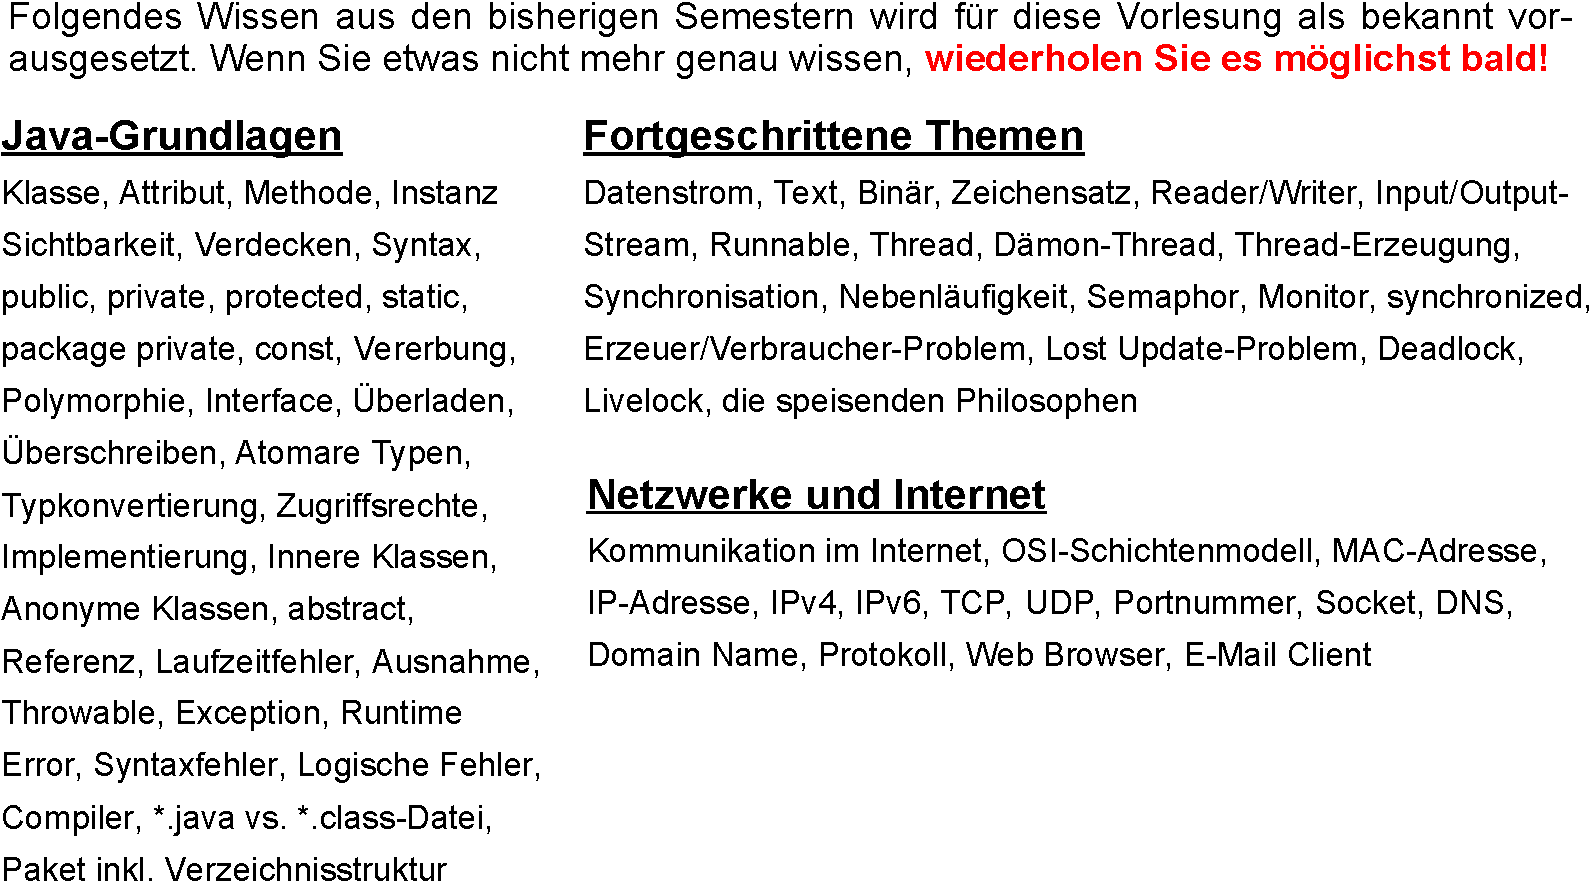
\includegraphics[width=\textwidth]{1-grundlagen/img/vorausgesetztes_wissen}
    \end{columns}
\end{frame}


%%% Folie
\begin{frame}{Benötigte Hard- und Software}
        \begin{columns}
            \begin{column}[T]{.5\textwidth}
                \textbf{Hardware}
                \medskip

                Wird von der DHBW zur Verfügung gestellt. Rückfrage, was genau
                angeschafft wurde, läuft gerade. \smiley{}
                \medskip

                \begin{itemize}
                    \item Raspberry Pi
                    \item Diverse Sensoren und Aktoren
                    \item \textcolor{gray}{Bildschirm, Tastatur, Maus für den Raspberry Pi}
                \end{itemize}
            \end{column}
            \begin{column}[T]{.5\textwidth}
                \textbf{Software}
                \medskip

                Eigentlich nicht viel. Das meiste ist unter Raspbian bereits
                installiert oder wird von uns im Laufe der Vorlesung ergänzt.
                Auf ihrem Laptop benötigen Sie ggf. noch folgende Programme:
                \medskip

                \begin{itemize}
                    \item OpenSSH / PuTTY für SSH-Verbindungen zum Pi
                    \item NetBeans und Maven für die Java-Programmierung
                    \item Python und Node.js als zusätzliche Sprachen
                \end{itemize}
            \end{column}
        \end{columns}
\end{frame}

%%% Folie
{
\small
\setlength{\fboxsep}{0pt}

\begin{frame}{Literaturempfehlungen}
    \begin{columns}
        \column[b]{.25\textwidth}
        \fbox{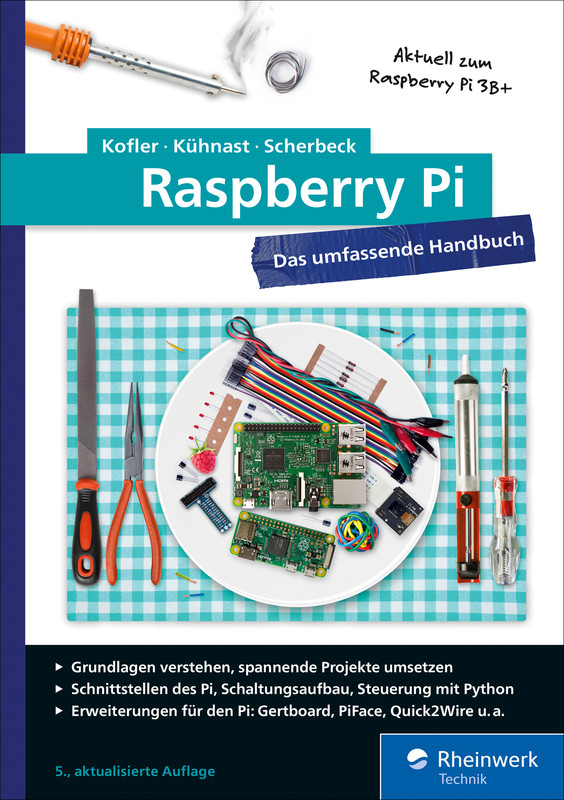
\includegraphics[height=3.8cm]{1-grundlagen/img/buch_raspberrypi}}

        \column[b]{.25\textwidth}
        \fbox{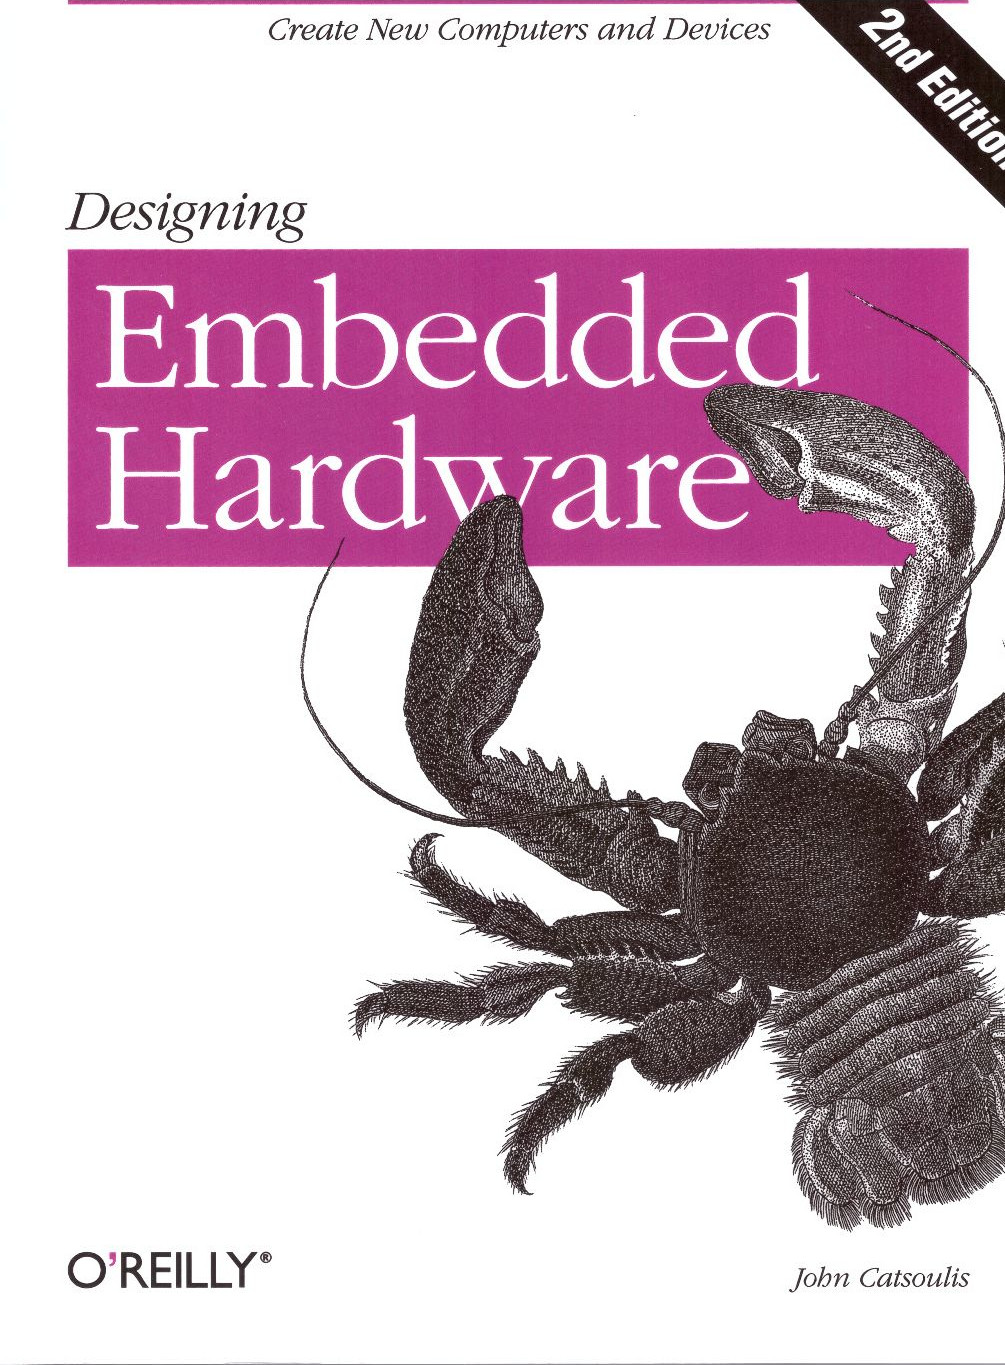
\includegraphics[height=3.8cm]{1-grundlagen/img/buch_embedded_hardware}}

        \column[b]{.25\textwidth}
        \fbox{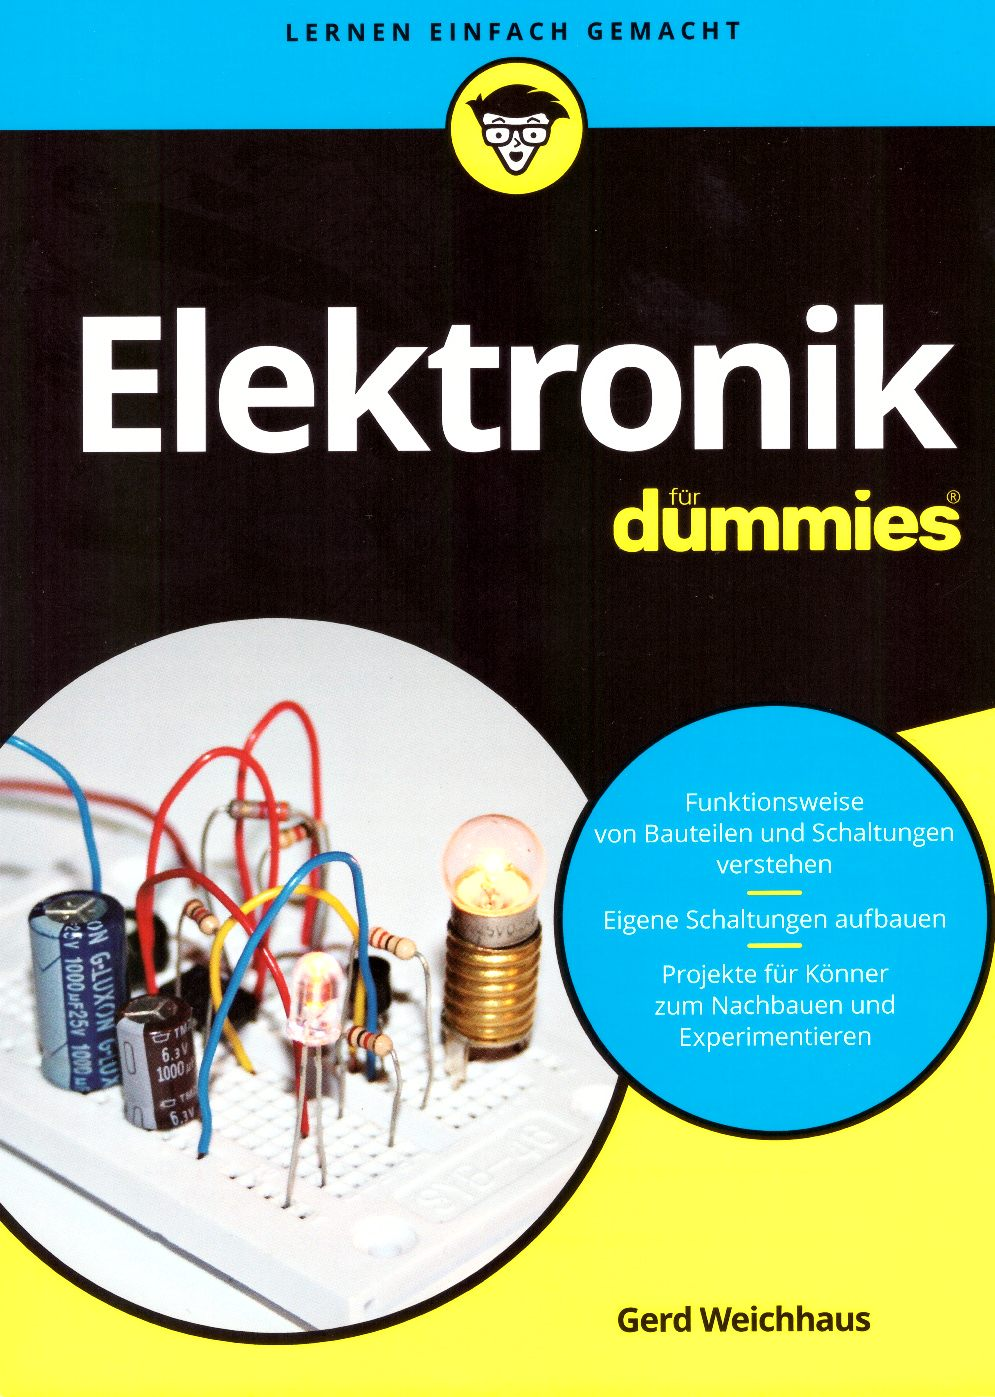
\includegraphics[height=3.8cm]{1-grundlagen/img/buch_elektronik_dummies}}

        \column[b]{.25\textwidth}
        \fbox{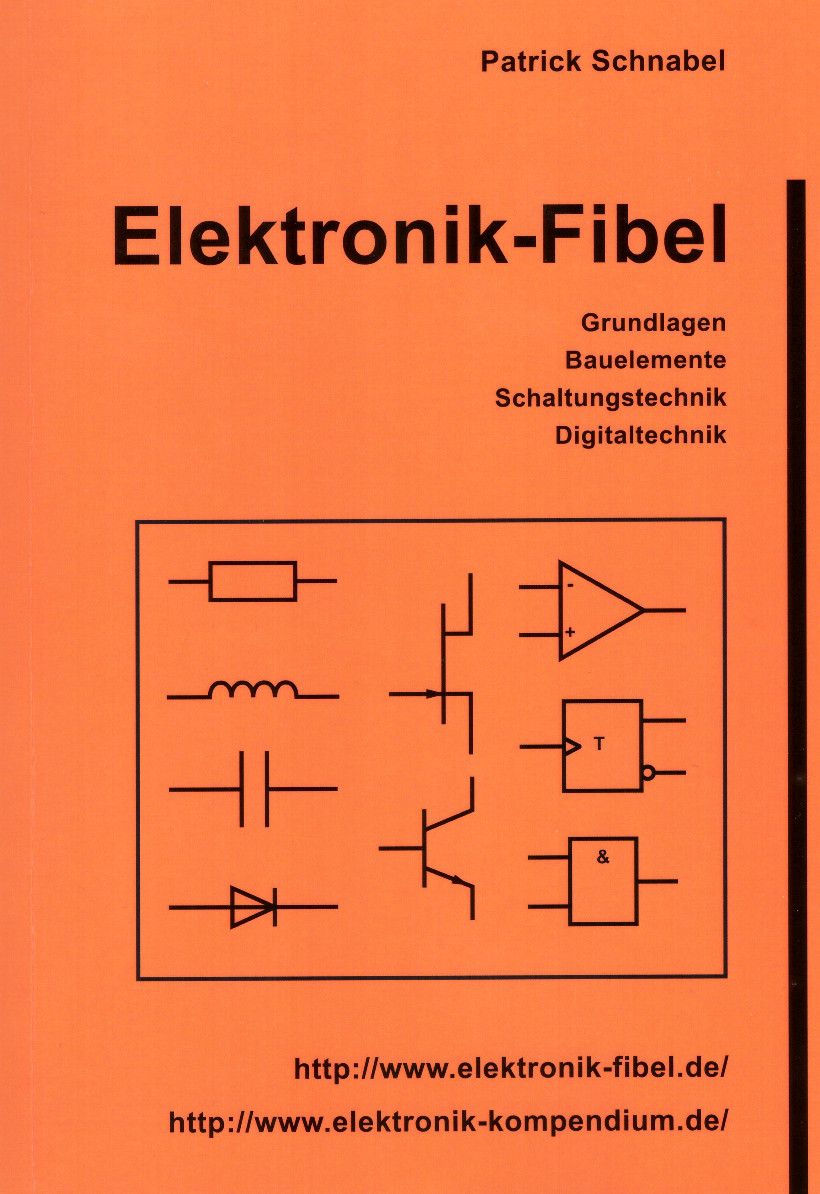
\includegraphics[height=3.8cm]{1-grundlagen/img/buch_elektronik_fibel}}
    \end{columns}

    \vskip 0.6cm

    \begin{columns}
        \column[T]{.5\textwidth}
        \textbf{Raspberry Pi: Das umfassende Handbuch für Maker und Tekkies} \\ Rheinwerk Verlag, 2018

        \column[T]{.5\textwidth}
        \textbf{Designing Embedded Hardware} \\ O'Reilly, 2005
    \end{columns}

    \vskip 0.6cm

    \begin{columns}
        \column[T]{.5\textwidth}
        \textbf{Elektronik für Dummies} \\ Wiley-VCH Verlag, 2018

        \column[T]{.5\textwidth}
        \textbf{Elektronik-Fibel} \\ Patrick Schnabel, 2017
    \end{columns}
\end{frame}
}

%%% Folie
\begin{frame}{Lernziele für heute}
    \begin{itemize}
        \item Die Bedeutung des Internet der Dinge in der heutigen Zeit verstehen
        \item Aktuelle IoT-Anwendungsfälle und Geschäftsprozesse erkennen
        \item ,,Internet of Things'' und ,,eingebettete Systeme'' voneinander abgrenzen
        \item Typische Schichten und Komponenten einer IoT-Architektur benennen
        \item Den aktuellen Stand der Technik im historischen Kontext einordnen
        \item Relevante Computerarchitekturen miteinander vergleichen
        \item Die Anforderungen an eingebettete Hard- und Software verstehen
    \end{itemize}
\end{frame}

%-------------------------------------------------------------------------------
\section{IoT-Anwendungsfälle}
%-------------------------------------------------------------------------------

%%% Folie
\begin{frame}{Embedded- und IoT-Devices im Alltag}
    \begin{columns}
        \column{\dimexpr\paperwidth-28pt}
        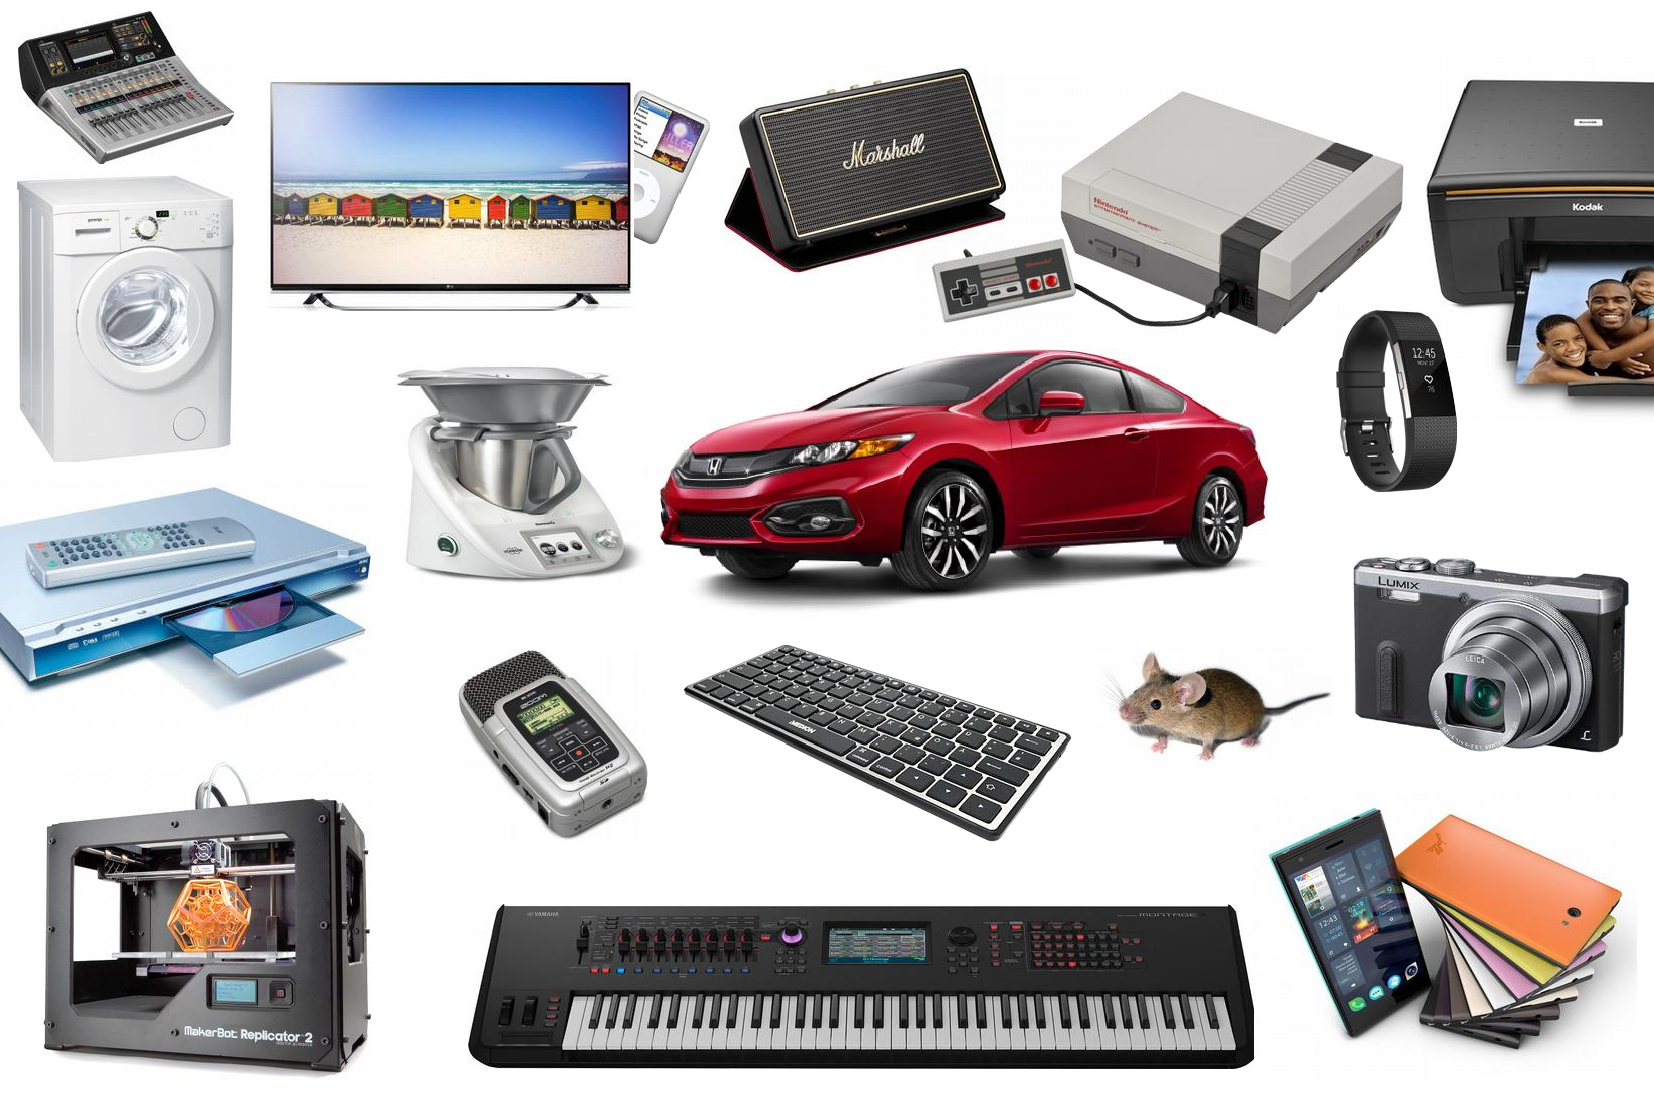
\includegraphics[width=\textwidth]{1-grundlagen/img/embedded_devices}
    \end{columns}
\end{frame}

%%% Folie
\begin{frame}{Embedded/IoT-Devices im Alltag}
    \begin{columns}
        \begin{column}[b]{.5\textwidth}
            \begin{center}
                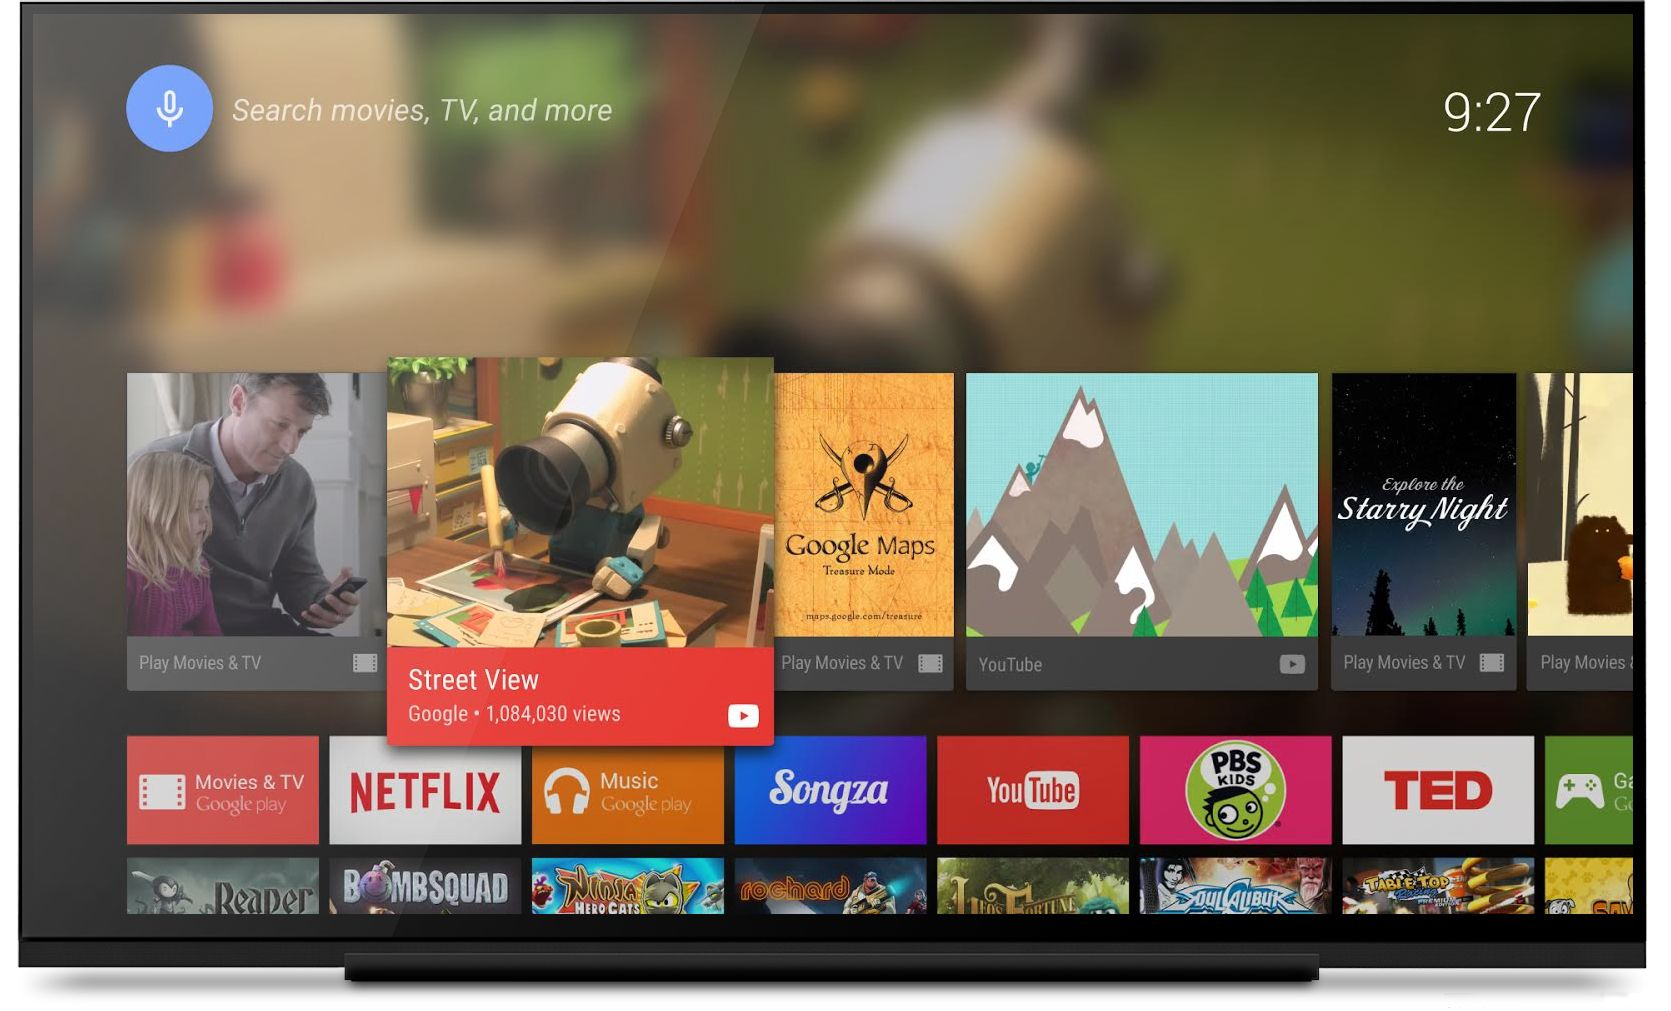
\includegraphics[width=\textwidth]{1-grundlagen/img/android_tv}
            \end{center}
        \end{column}
        \begin{column}[b]{.5\textwidth}
            \begin{center}
                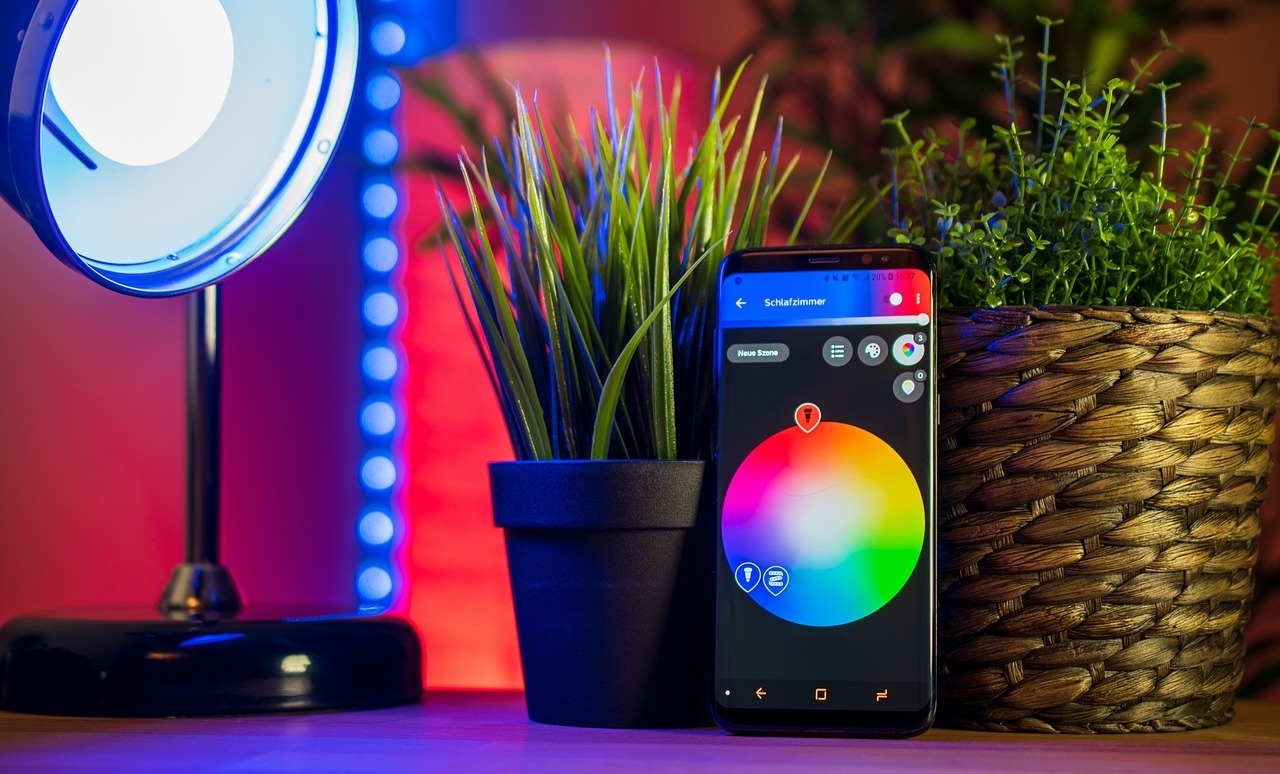
\includegraphics[width=\textwidth]{1-grundlagen/img/smart-home-3779361_1280}
            \end{center}
        \end{column}
    \end{columns}

    \bigskip

    \begin{itemize}
        \item Was bedeutet der Begriff „Internet of Things“?
        \item Was macht ein Device zu einem IoT-Device?
        \item Wie unterscheidet es sich von gewöhnlichen Embedded-Devices?
        \item Welche Anwendungsfälle für IoT können Sie sich vorstellen?
    \end{itemize}
\end{frame}

%%% Folie
\begin{frame}{Industrielle IoT-Anwendungsfälle}
    \textbf{Smight -- Smart City Light}
    \hfill
    \Href{https://smight.com/}
    \medskip
    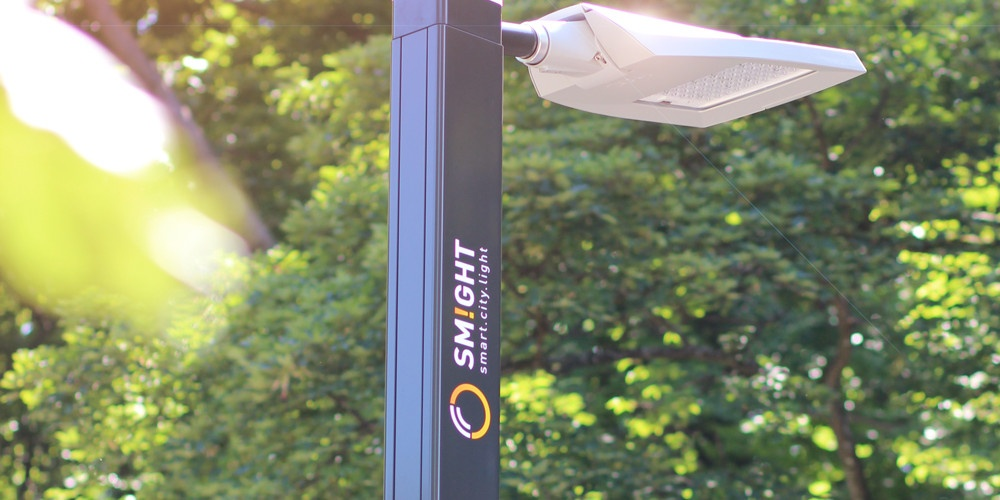
\includegraphics[width=0.49\textwidth]{1-grundlagen/img/smight1}
    \hfill
    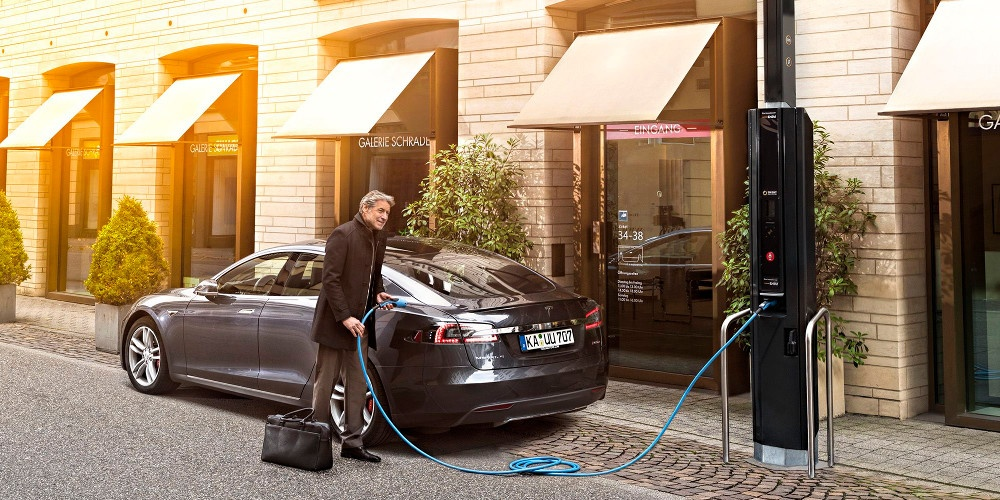
\includegraphics[width=0.49\textwidth]{1-grundlagen/img/smight2}

    \bigskip

    \textbf{Testfeld autonomes Fahren Baden-Württemberg}
    \hfill
    \Href{https://taf-bw.de/}
    \medskip
    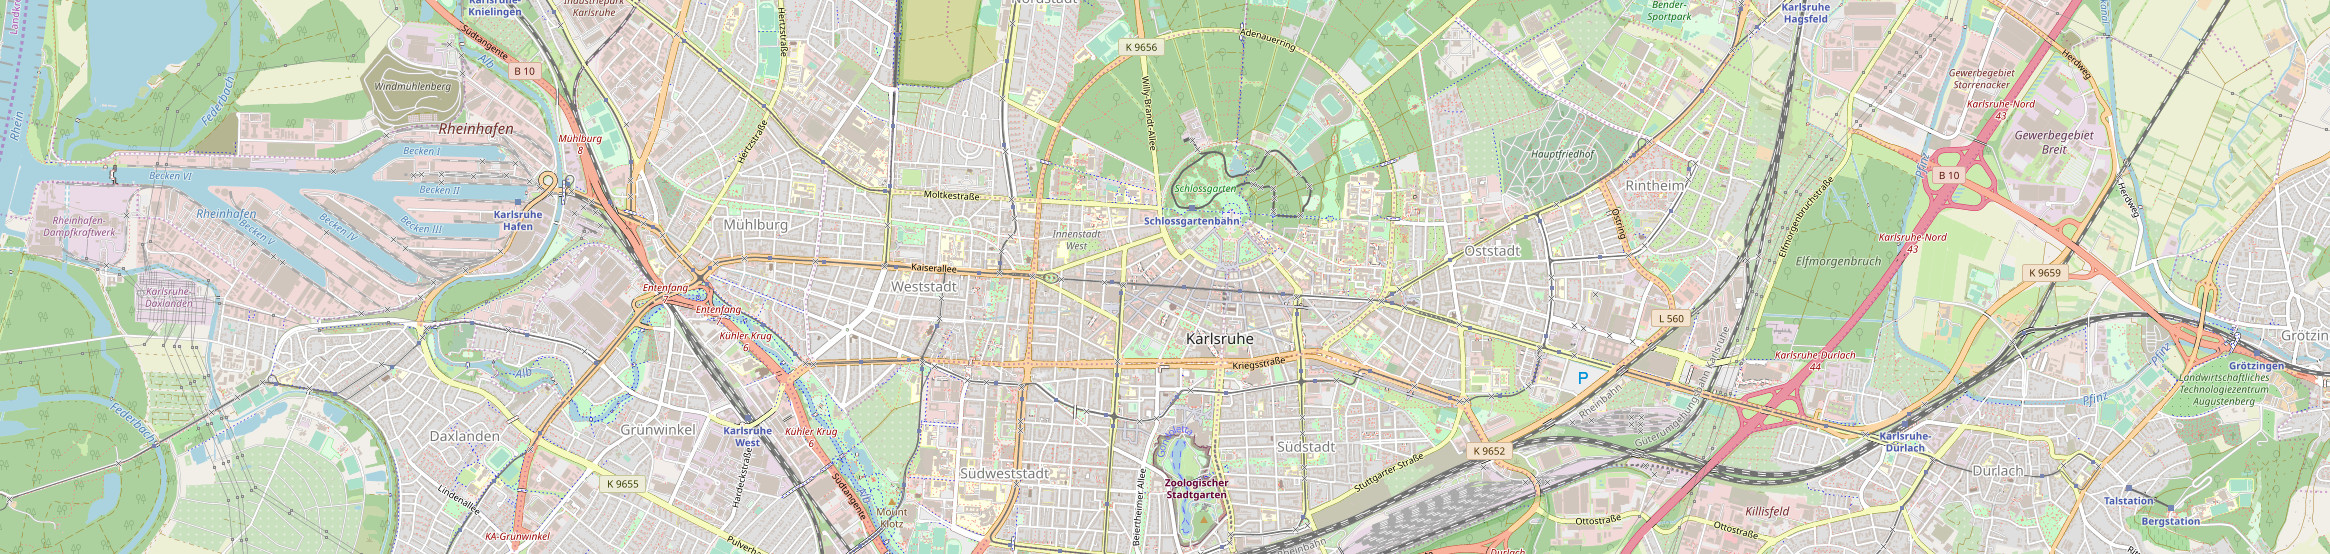
\includegraphics[width=\textwidth]{1-grundlagen/img/karlsruhe}
\end{frame}

%-------------------------------------------------------------------------------
\section{Technische Grundlagen}
%-------------------------------------------------------------------------------

{
\small

%%% Folie
\begin{frame}{Definition ,,Eingebettetes Computersystem''}
    \begin{block}{Definition}
        \parbox{\linewidth}{
            \smallskip

            Eingebettete Systeme sind kleine Mikrocomputer, die innerhalb eines größeren Geräts
            meist unsichtbar verbaut sind, um seine Funktionen zu steuern und überwachen. In vielen
            Fällen geben sie einem Gerät überhaupt erst seine Funktion, ohne dass dies für den
            Anwender offensichtlich ist.
            \smallskip

            Ihre grundsätzliche Architektur ist dieselbe wie bei konventionellen Computern,
            jedoch verfügen sie über weitaus weniger, genau auf den Anwendungsfall zugeschnittene
            Ressourcen bei minimalen Kosten, Platzbedarf und Energieverbrauch. Der Leitgedanke
            hierbei lautet ,,so viel wie gerade nötig, so wenig wie absolut möglich''.
            Eingebettete Systeme sind meist in sich geschlossene Systeme mit deterministischem
            Systemverhalten, die rund um die Uhr laufen und exakt eine Aufgabe erfüllen.
        }
    \end{block}

    \begin{block}{Beispiele}
        \begin{columns}[onlytextwidth]
            \column[b]{.2\textwidth}
            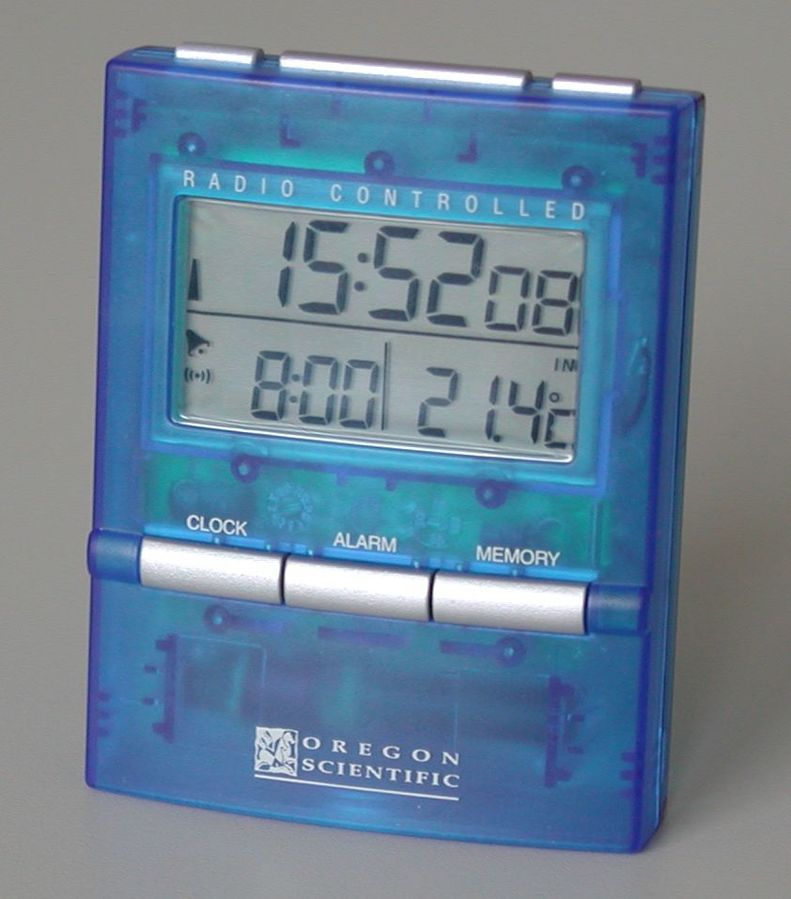
\includegraphics[width=\textwidth]{1-grundlagen/img/funkwecker}

            \column[b]{.2\textwidth}
            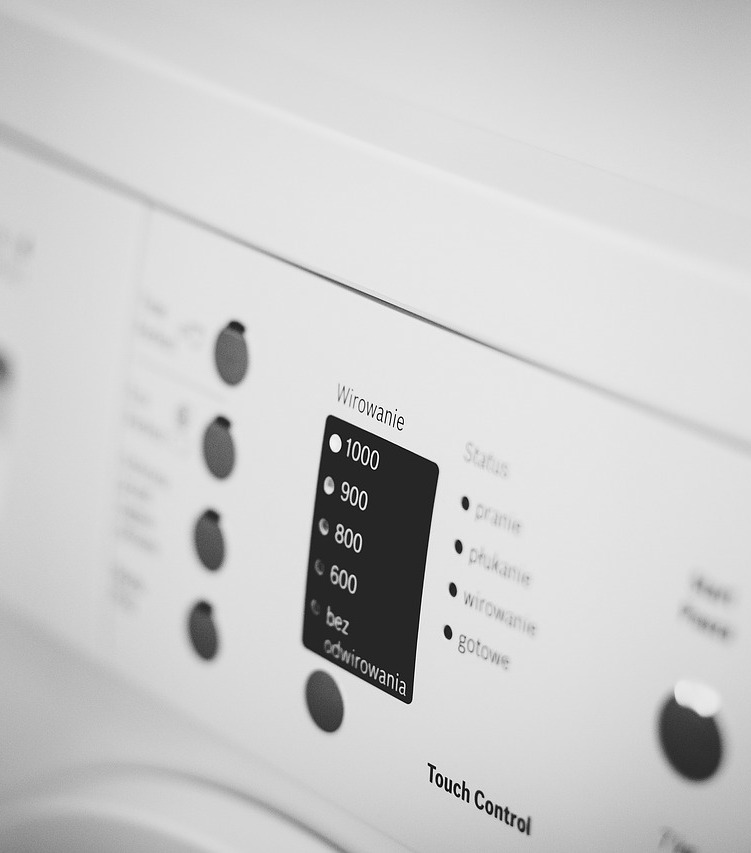
\includegraphics[width=\textwidth]{1-grundlagen/img/washing-machine-2617514_1280}

            \column[b]{.2\textwidth}
            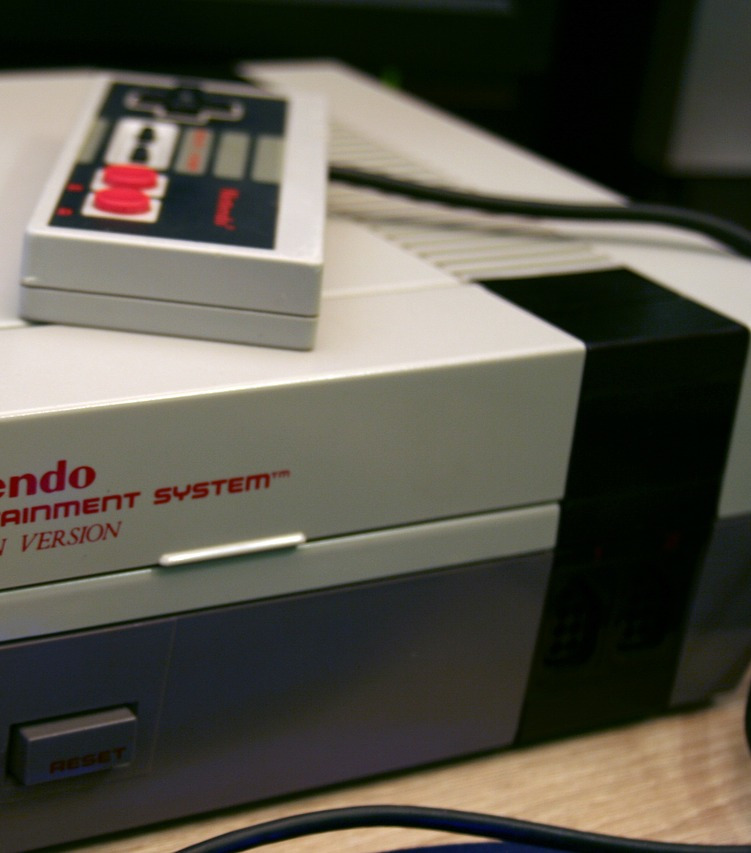
\includegraphics[width=\textwidth]{1-grundlagen/img/nes-2649705_1280}

            \column[b]{.2\textwidth}
            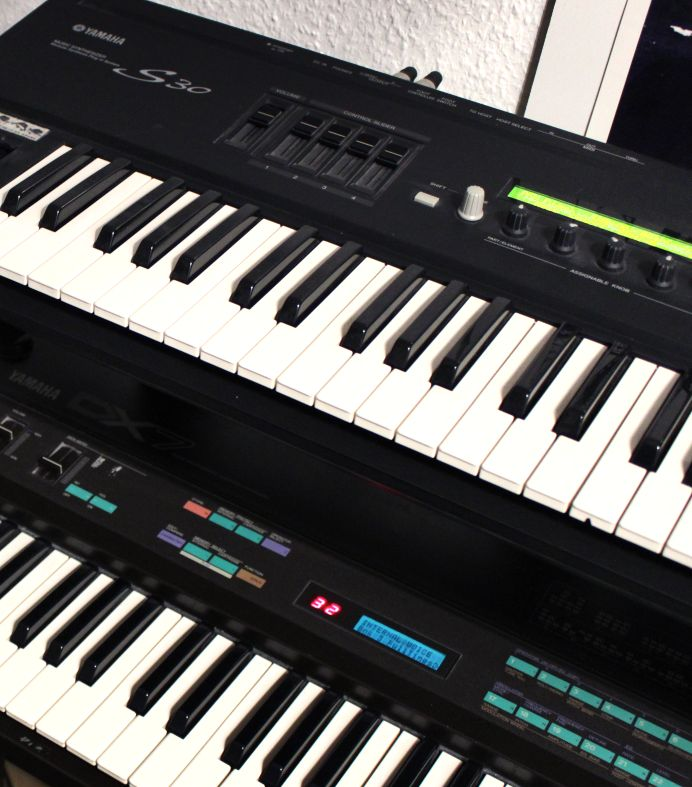
\includegraphics[width=\textwidth]{1-grundlagen/img/keyboards}

            \column[b]{.2\textwidth}
            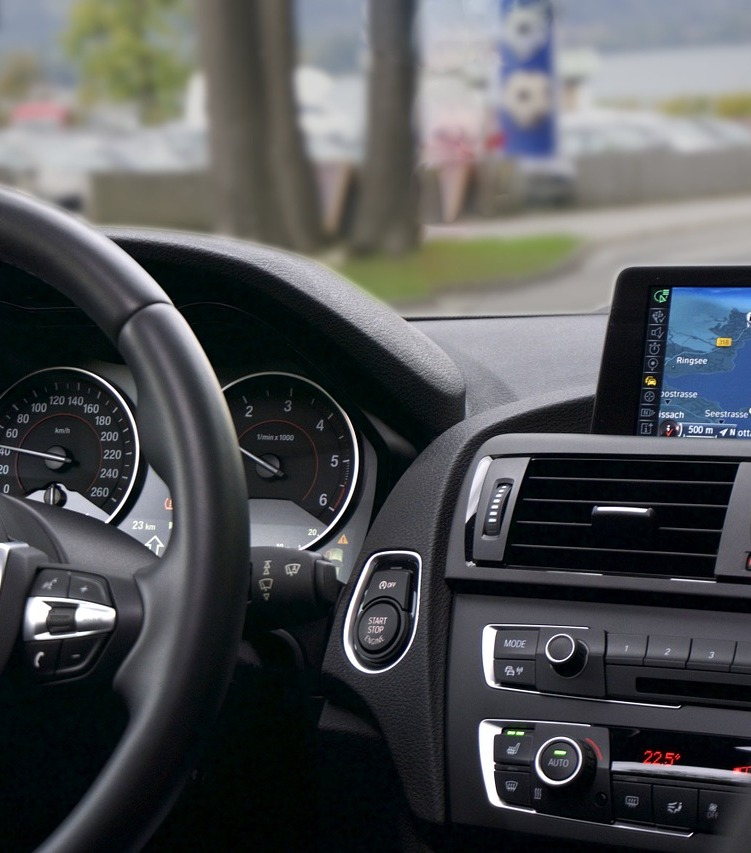
\includegraphics[width=\textwidth]{1-grundlagen/img/car-1281640_1280}
        \end{columns}
    \end{block}
\end{frame}

%%% Folie
\begin{frame}{Definition ,,Internet of Things''}
    \begin{block}{Definition}
        \parbox{\linewidth}{
            \smallskip

            IoT-Devices sind eine Teilmenge eingebetteter Systeme größerer Leistungsklasse mit
            permanenter Internetverbindung. Die ursprüngliche Definition aus dem Jahr 1999
            sah die eindeutige, maschinenlesbare Identifikation physischer Objekte anhand von
            RFID-Tags vor. Heute versteht man darunter an einem physischen Objekt angebrachte,
            direkt mit dem Internet verbundene und über ihre IP-Adresse identifizierte Kleinstcomputer,
            da diese inzwischen auf wenigen Quadratzentimetern Platz finden.
            \smallskip

            Im erweiterten Sinne zählen zum ,,Internet of Things'' heute auch Infrastruktur, Cloud-
            und Backendservices, über welche die Devices miteinander verbunden, verwaltet, gesteuert
            und überwacht werden können.
        }
    \end{block}

    \medskip
    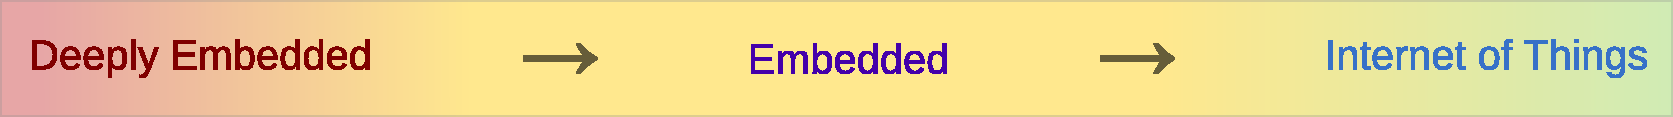
\includegraphics[width=\textwidth]{1-grundlagen/img/embedded_typen}

    \begin{block}{Beispiele}
        \begin{columns}[onlytextwidth]
            \column[b]{.33\textwidth}
            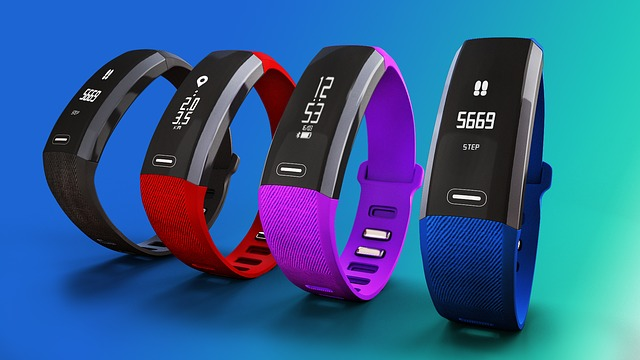
\includegraphics[width=\textwidth]{1-grundlagen/img/heart-rate-monitoring-device-1903997_640}

            \column[b]{.33\textwidth}
            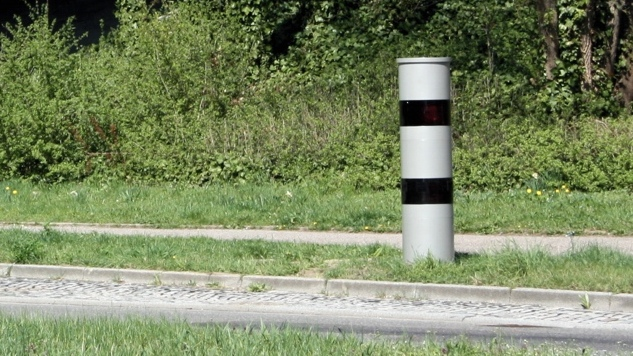
\includegraphics[width=\textwidth]{1-grundlagen/img/blitzer_pulverhausstrasse}

            \column[b]{.33\textwidth}
            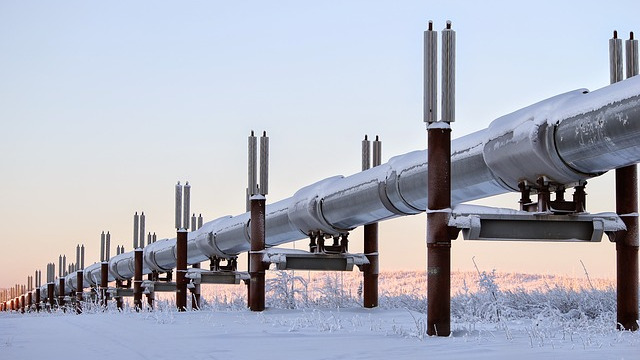
\includegraphics[width=\textwidth]{1-grundlagen/img/winter-681175_640}
        \end{columns}
    \end{block}
\end{frame}
}

%%% Folie
{
\setbeamertemplate{background canvas}{
    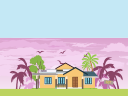
\includegraphics[height=\paperheight, width=\paperwidth]{1-grundlagen/img/themengebiete1}
}

\begin{frame}[fragile]{IoT -- Ein Haus mit tiefem Keller}
    \only<beamer:2|handout:0>{
        \transdissolve

        \begin{tikzpicture}[remember picture,overlay]
            \node at (5.4cm,0.28cm){
                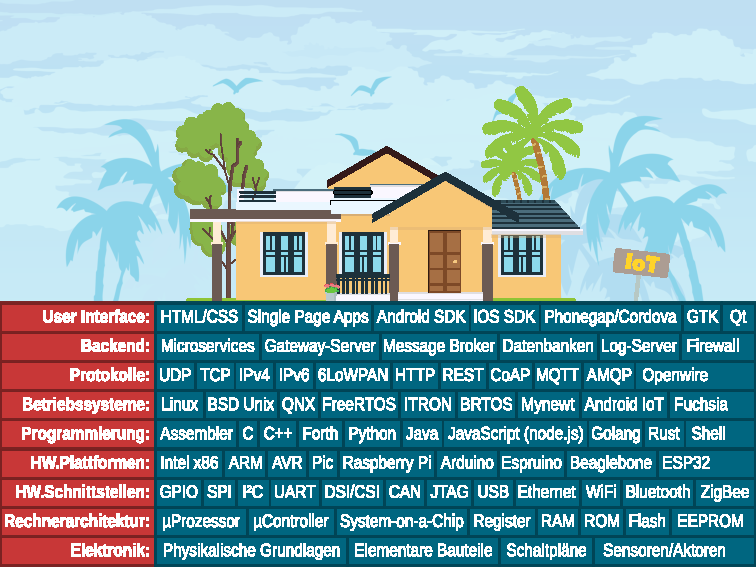
\includegraphics[height=\paperheight, width=\paperwidth]{1-grundlagen/img/themengebiete2}
            };
        \end{tikzpicture}
    }

    \only<beamer:3|handout:0>{
        \transdissolve

        \begin{tikzpicture}[remember picture,overlay]
            \node at (5.4cm,0.28cm){
                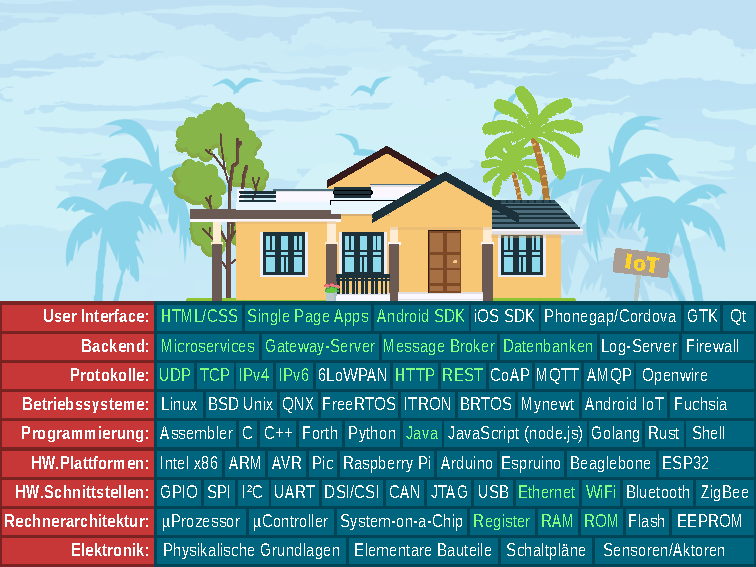
\includegraphics[height=\paperheight, width=\paperwidth]{1-grundlagen/img/themengebiete3}
            };
        \end{tikzpicture}
    }

    \only<beamer:4|handout:0>{
        \transdissolve

        \begin{tikzpicture}[remember picture,overlay]
            \node at (5.4cm,0.28cm){
                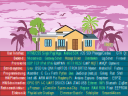
\includegraphics[height=\paperheight, width=\paperwidth]{1-grundlagen/img/themengebiete4}
            };
        \end{tikzpicture}
    }
\end{frame}
}

{
\setbeamertemplate{background canvas}{
    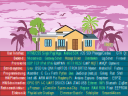
\includegraphics[height=\paperheight, width=\paperwidth]{1-grundlagen/img/themengebiete4}
}

\begin{frame}<handout>[plain]
\end{frame}
}

%%% Folie
\begin{frame}{Beispiel einer typischen IoT-Architektur}
    \begin{columns}
        \column{\dimexpr\paperwidth-10pt}
        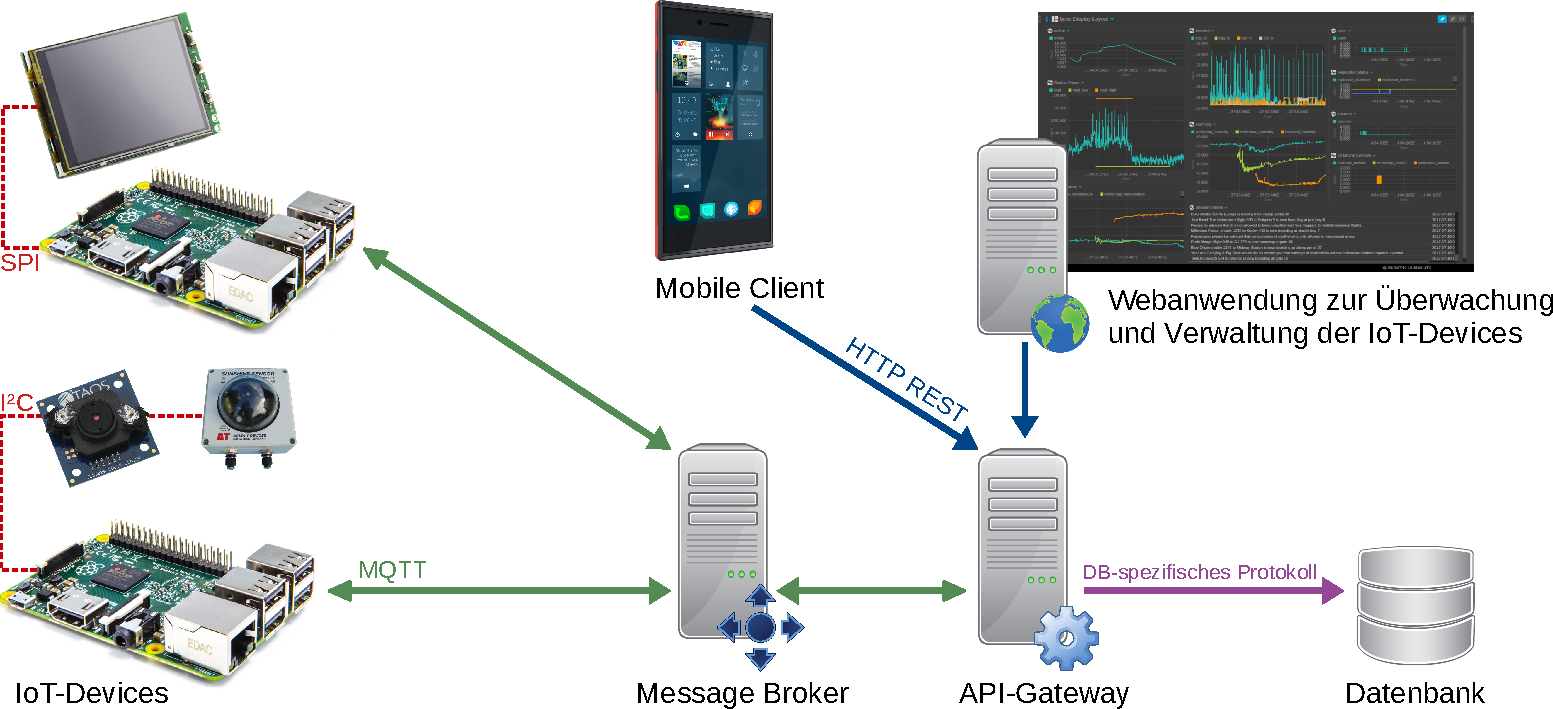
\includegraphics[width=\textwidth]{1-grundlagen/img/architektur_beispiel}
    \end{columns}
\end{frame}

%%% Folie
\begin{frame}[allowframebreaks]{Eine kleine Computer-Geschichte}
    \begin{columns}
        \column{\dimexpr\paperwidth-10pt}
        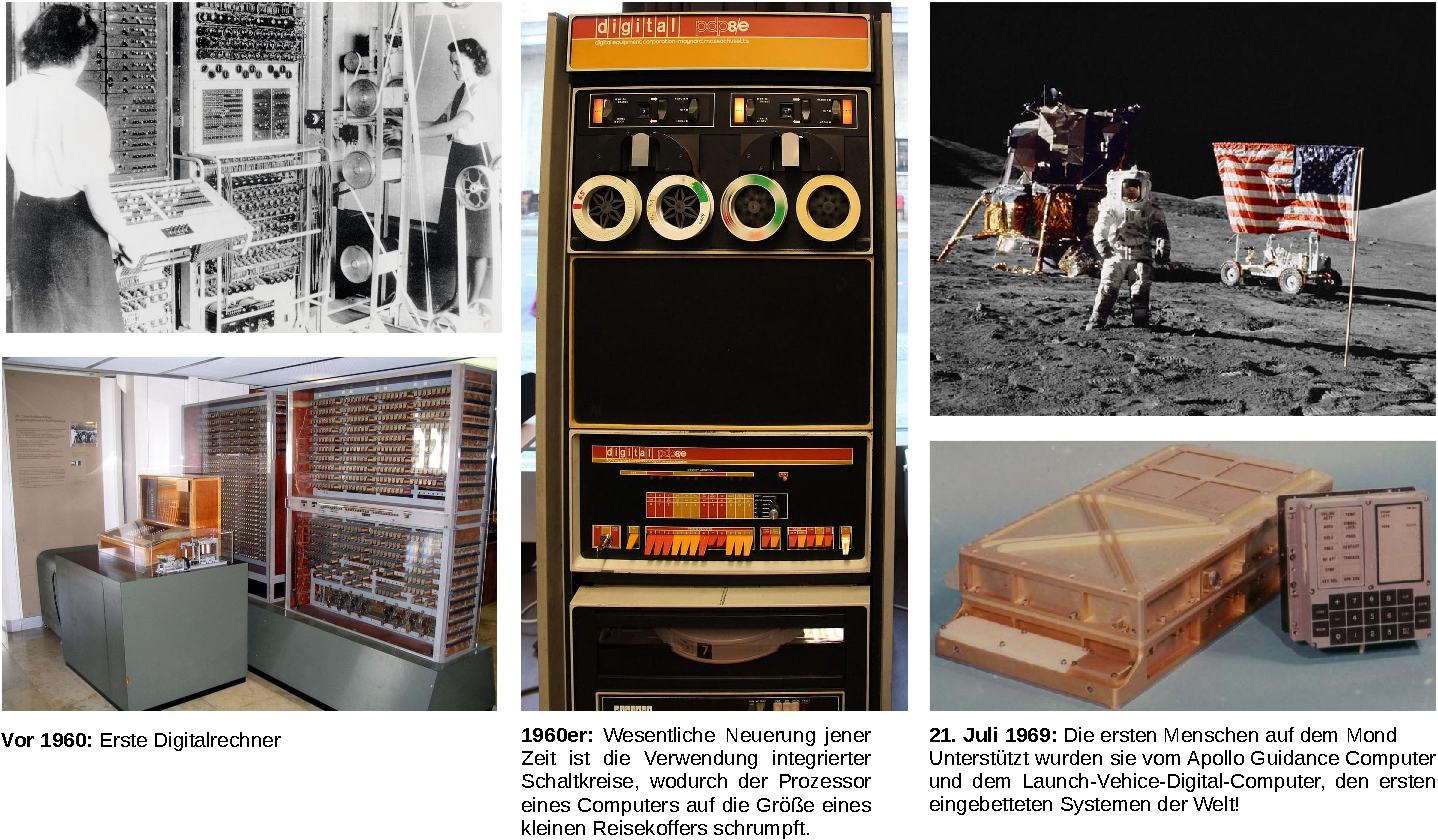
\includegraphics[width=\textwidth]{1-grundlagen/img/geschichte1}
    \end{columns}

    \begin{columns}
        \column{\dimexpr\paperwidth-10pt}
        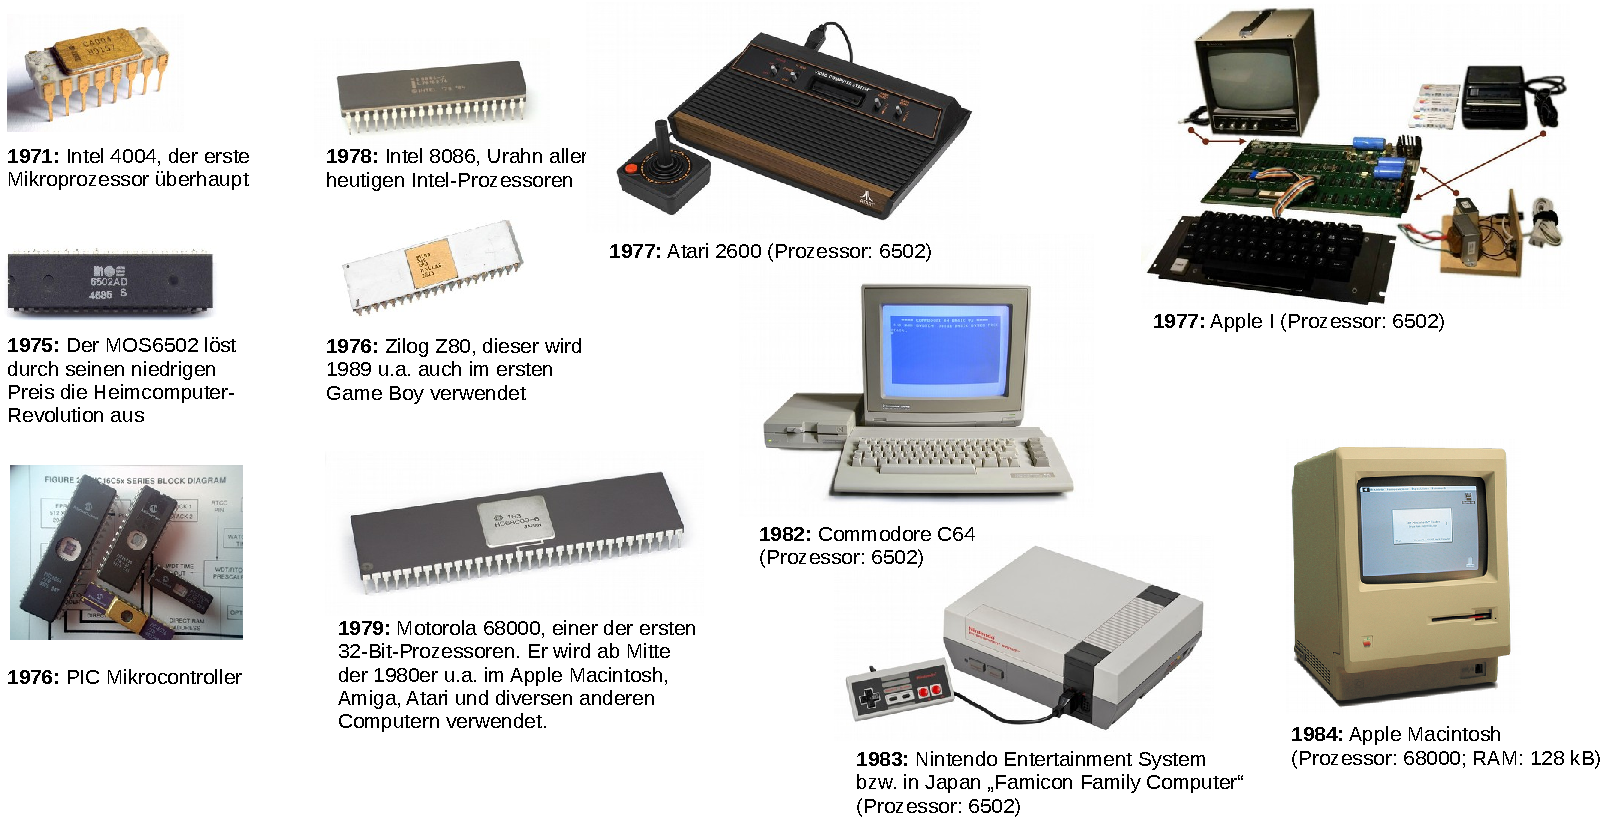
\includegraphics[width=\textwidth]{1-grundlagen/img/geschichte2}
    \end{columns}

    \begin{columns}
        \column{\dimexpr\paperwidth-10pt}
        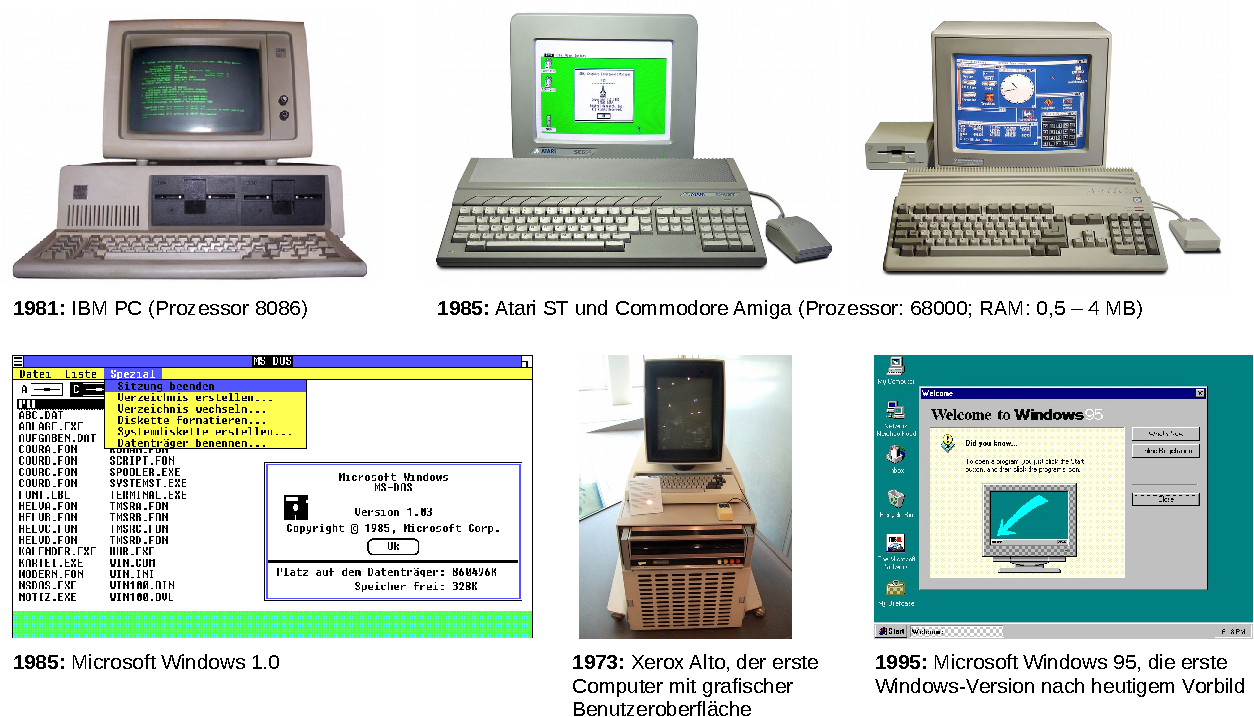
\includegraphics[width=\textwidth]{1-grundlagen/img/geschichte3}
    \end{columns}

    \begin{columns}
        \column{\dimexpr\paperwidth-10pt}
        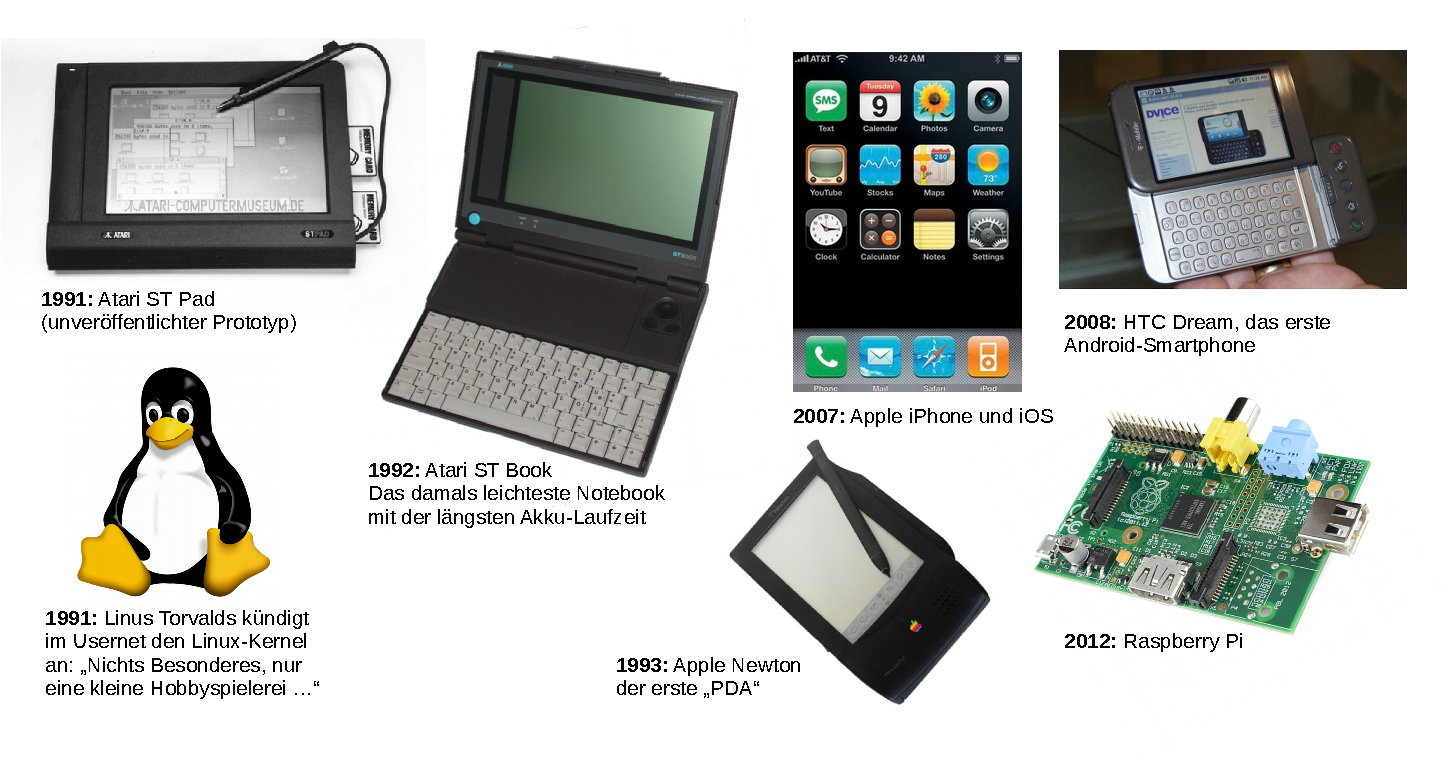
\includegraphics[width=\textwidth]{1-grundlagen/img/geschichte4}
    \end{columns}
\end{frame}

%%% Folie
\begin{frame}{Minimale Grundkomponenten eines Computers}
    \only<beamer:1|handout:0>{
        \begin{center}
            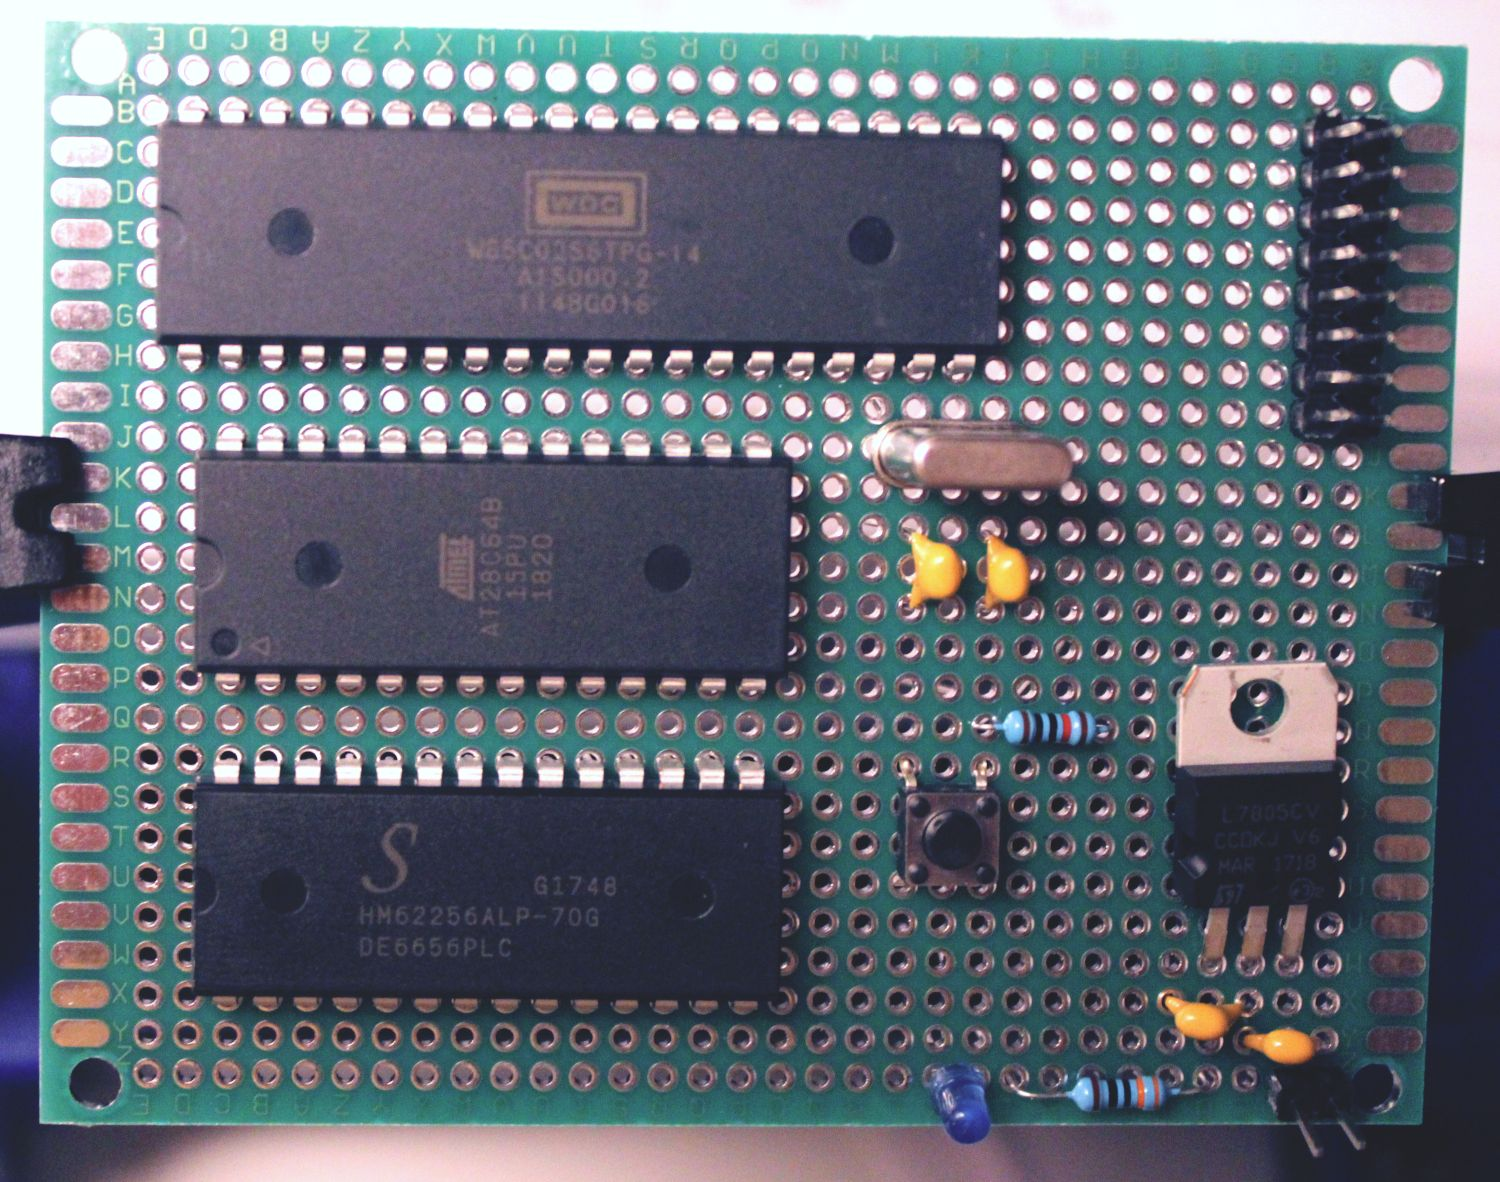
\includegraphics[height=0.85\textheight]{1-grundlagen/img/sbc_microprozessor1_klein}
        \end{center}
    }

    \only<2>{
        \begin{center}
            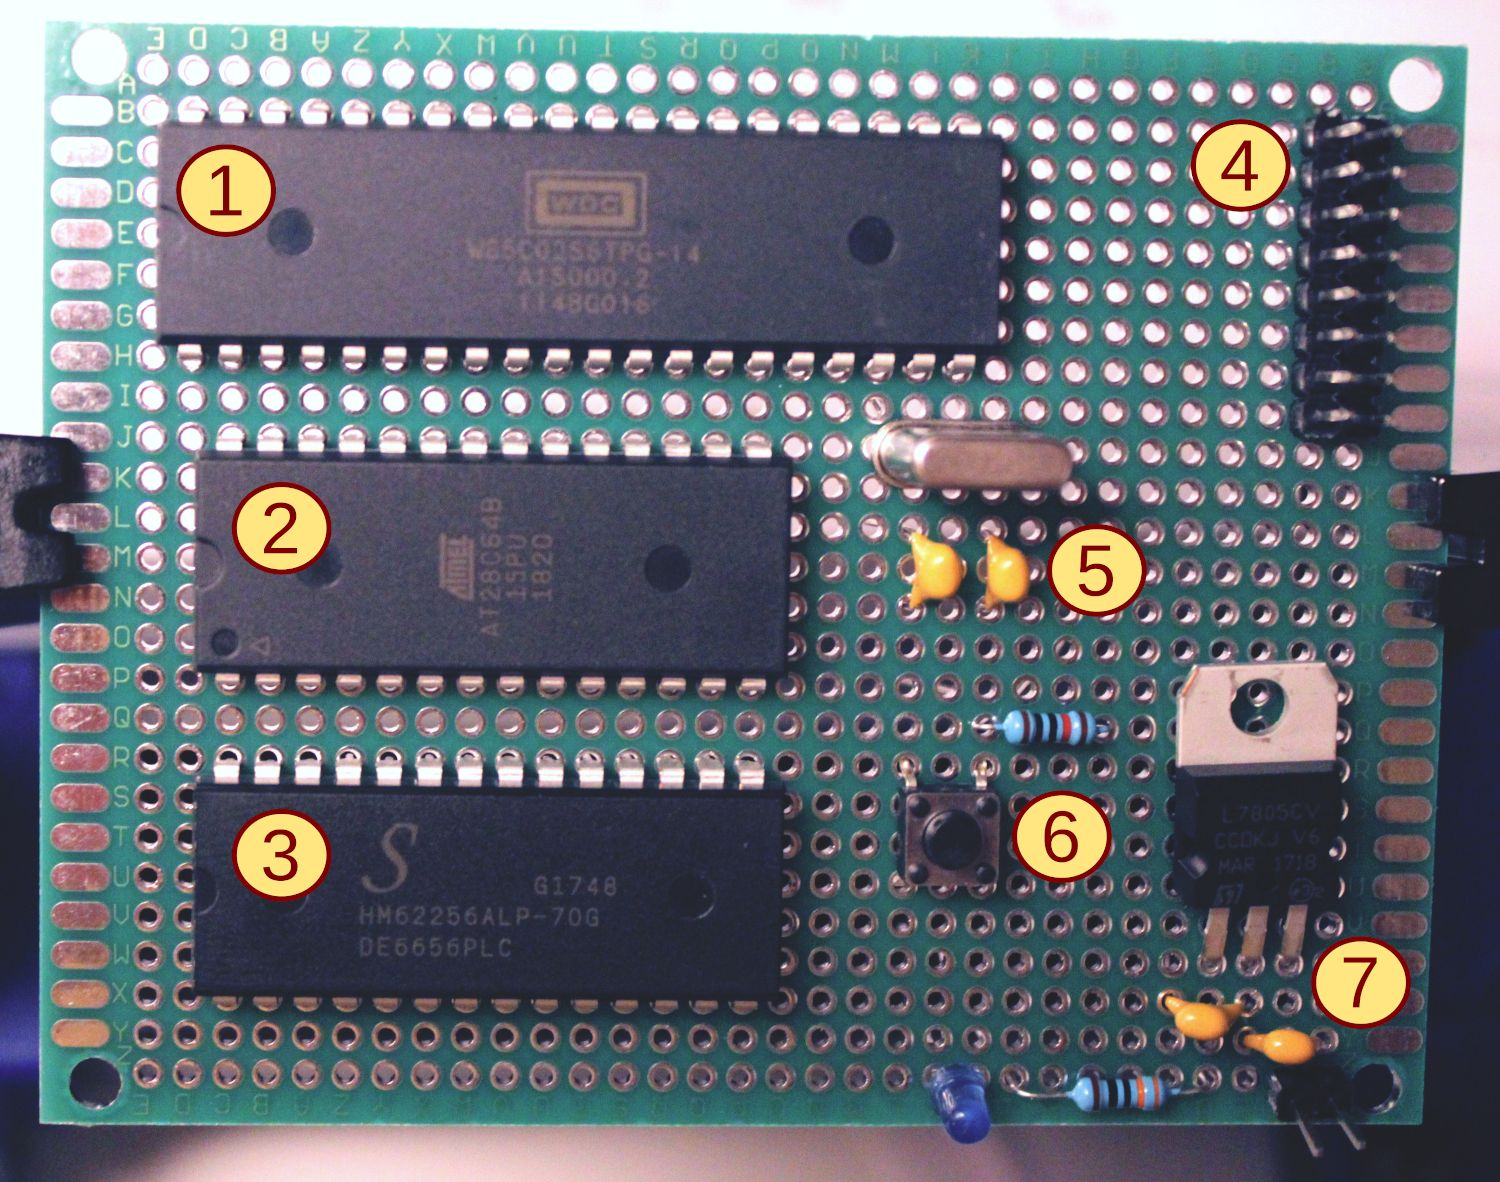
\includegraphics[height=0.5\textheight]{1-grundlagen/img/sbc_microprozessor2_klein}
        \end{center}

        \medskip

        \begin{columns}
            \begin{column}[T]{.5\textwidth}
                \textbf{Digitale Bausteine}
                \begin{enumerate}
                    \item Mikroprozessor
                    \item Programmspeicher
                    \item Hauptspeicher
                    \item I/O-Ports
                \end{enumerate}
            \end{column}
            \begin{column}[T]{.5\textwidth}
                \textbf{Hilfsschaltungen}
                \begin{enumerate}
                    \setcounter{enumi}{4}
                    \item Taktgeber
                    \item Resetschalter
                    \item Stromversorgung
                \end{enumerate}
            \end{column}
        \end{columns}
    }
\end{frame}

%%% Folie
{
    \setbeamertemplate{background canvas}{
        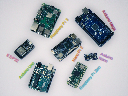
\includegraphics[height=\paperheight, width=\paperwidth]{1-grundlagen/img/sbc_auswahl}
    }

    \begin{frame}[plain]
        \transdissolve

        \only<beamer:2|handout:0>{
            \transdissolve

            \begin{tikzpicture}[remember picture,overlay]
                \node at (5.4cm,-0.97cm){
                    \includegraphics[height=\paperheight, width=\paperwidth]{1-grundlagen/img/bauteile}
                };
            \end{tikzpicture}
        }
    \end{frame}
}{
    \setbeamertemplate{background canvas}{
        \includegraphics[height=\paperheight, width=\paperwidth]{1-grundlagen/img/bauteile}
    }

    \begin{frame}<handout>[plain]
        \transdissolve
    \end{frame}
}

%%% Folie
\begin{frame}{Fallbeispiel: Laufschrift mit Raspberry Pi und Arduino}
    \begin{columns}
        \column[b]{.5\textwidth}
        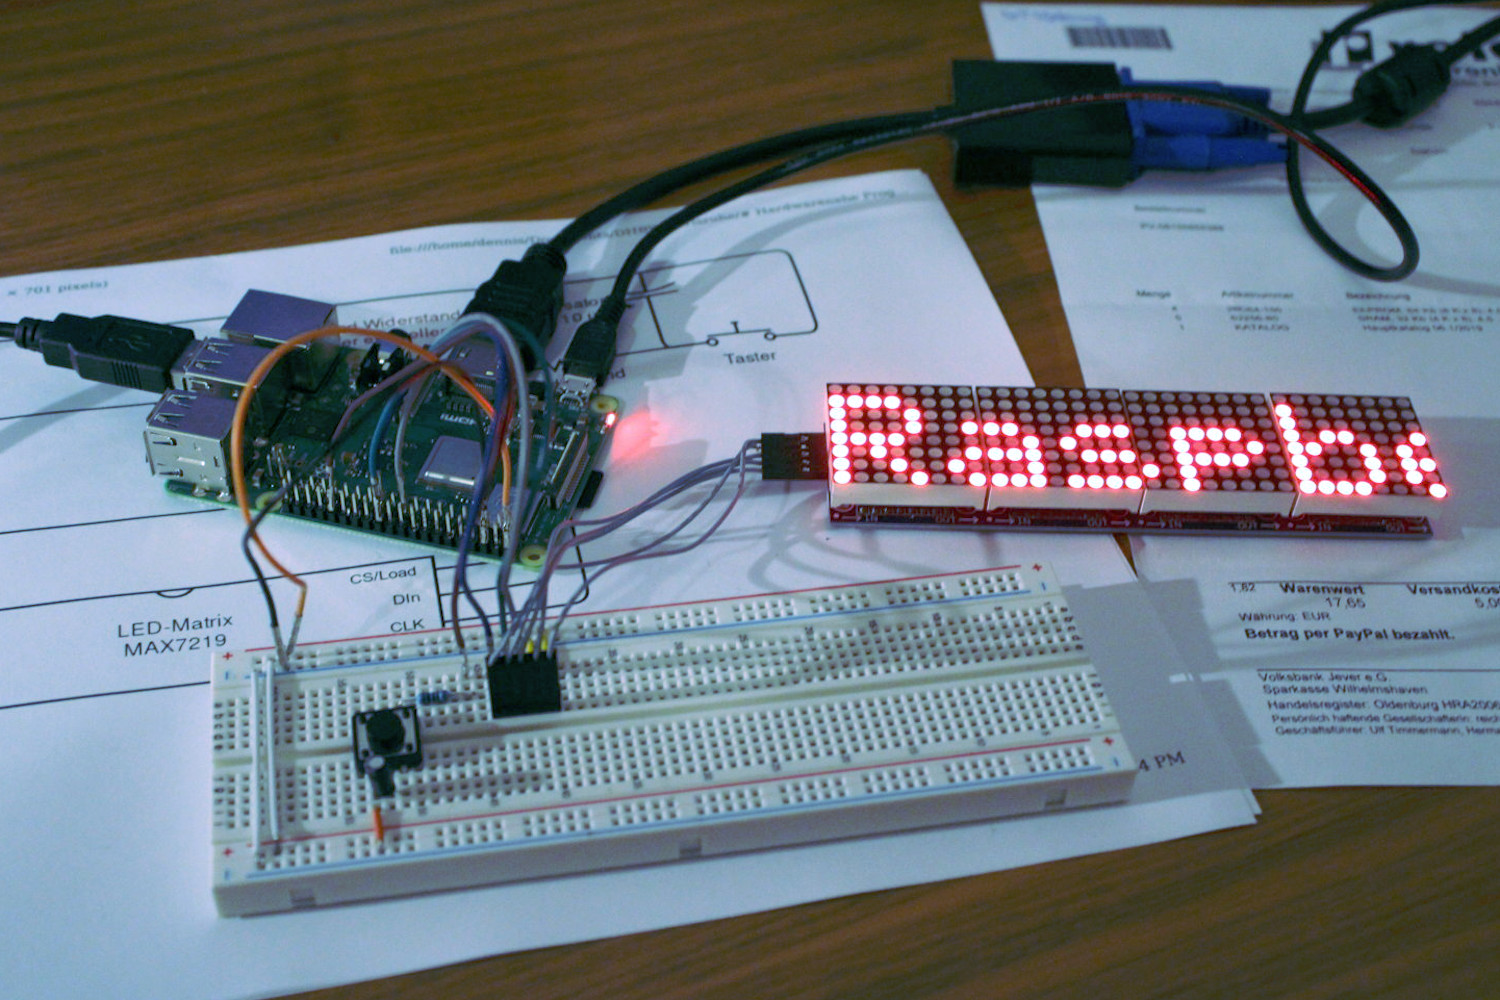
\includegraphics[width=\textwidth]{1-grundlagen/img/laufschrift_pi1}

        \column[b]{.5\textwidth}
        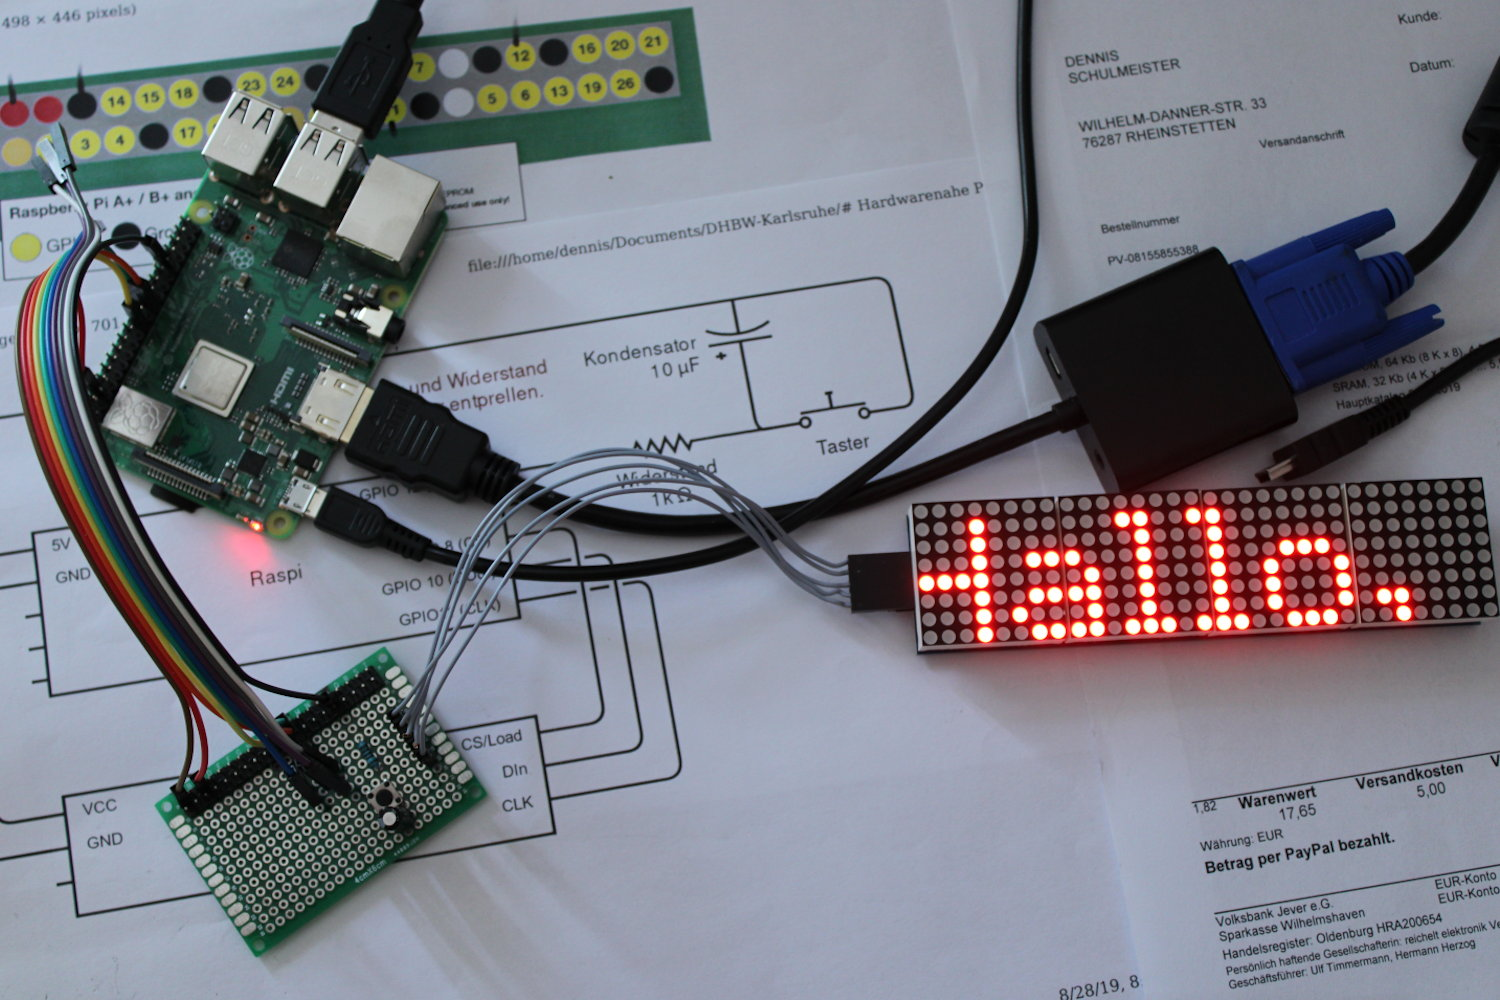
\includegraphics[width=\textwidth]{1-grundlagen/img/laufschrift_pi2}
    \end{columns}

    \medskip

    \begin{columns}
        \column[b]{.5\textwidth}
        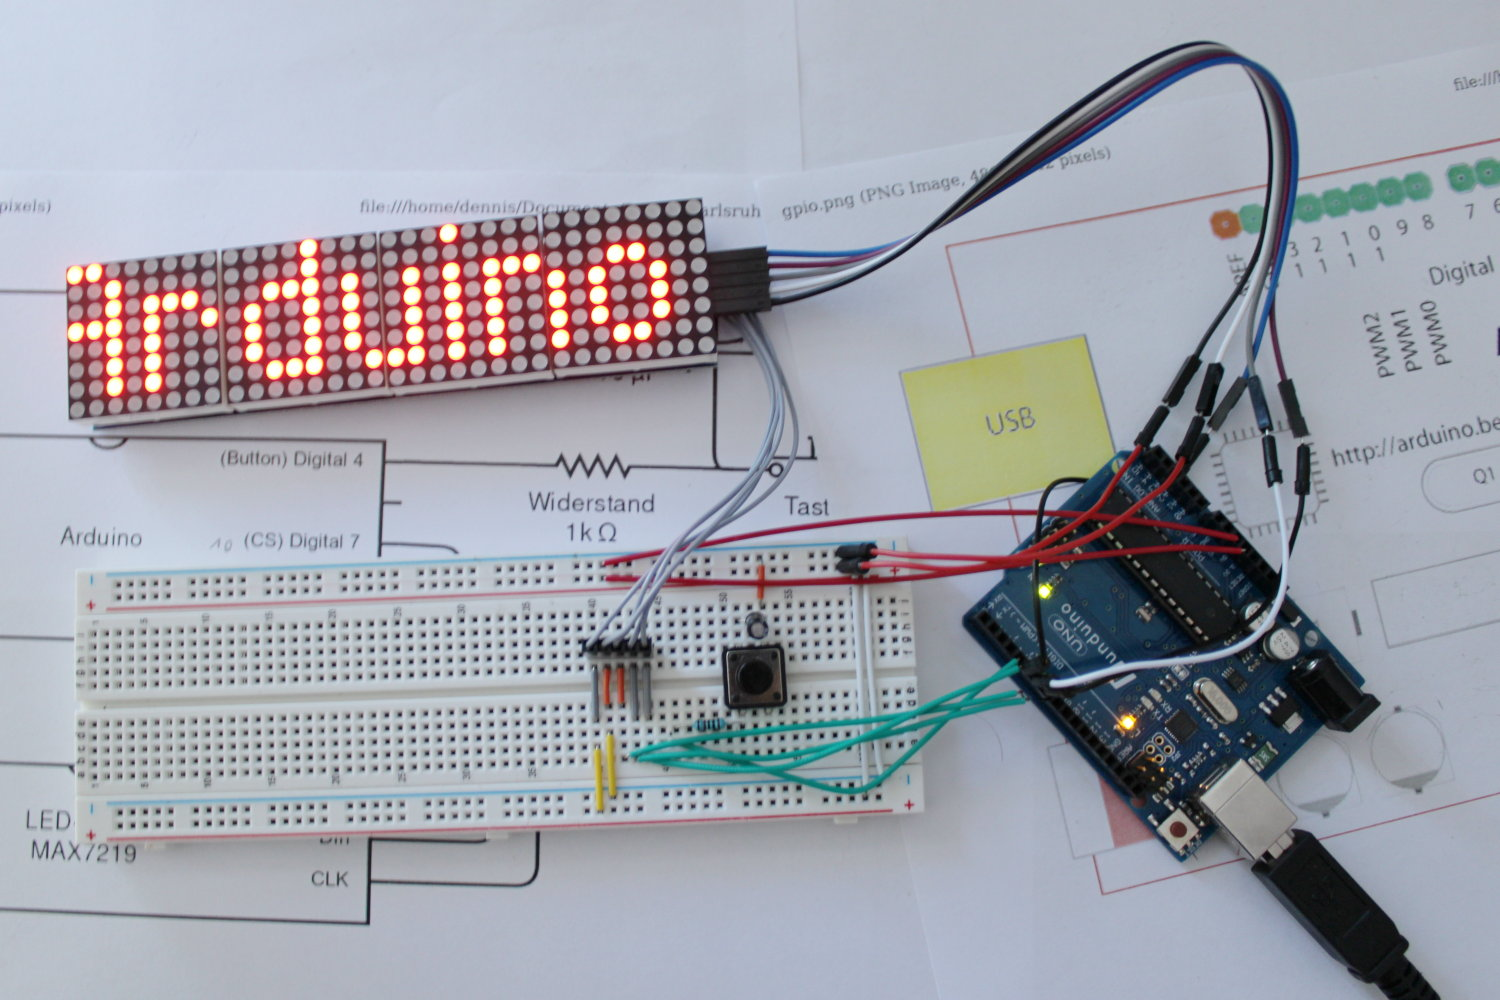
\includegraphics[width=\textwidth]{1-grundlagen/img/laufschrift_arduino1}

        \column[b]{.5\textwidth}
        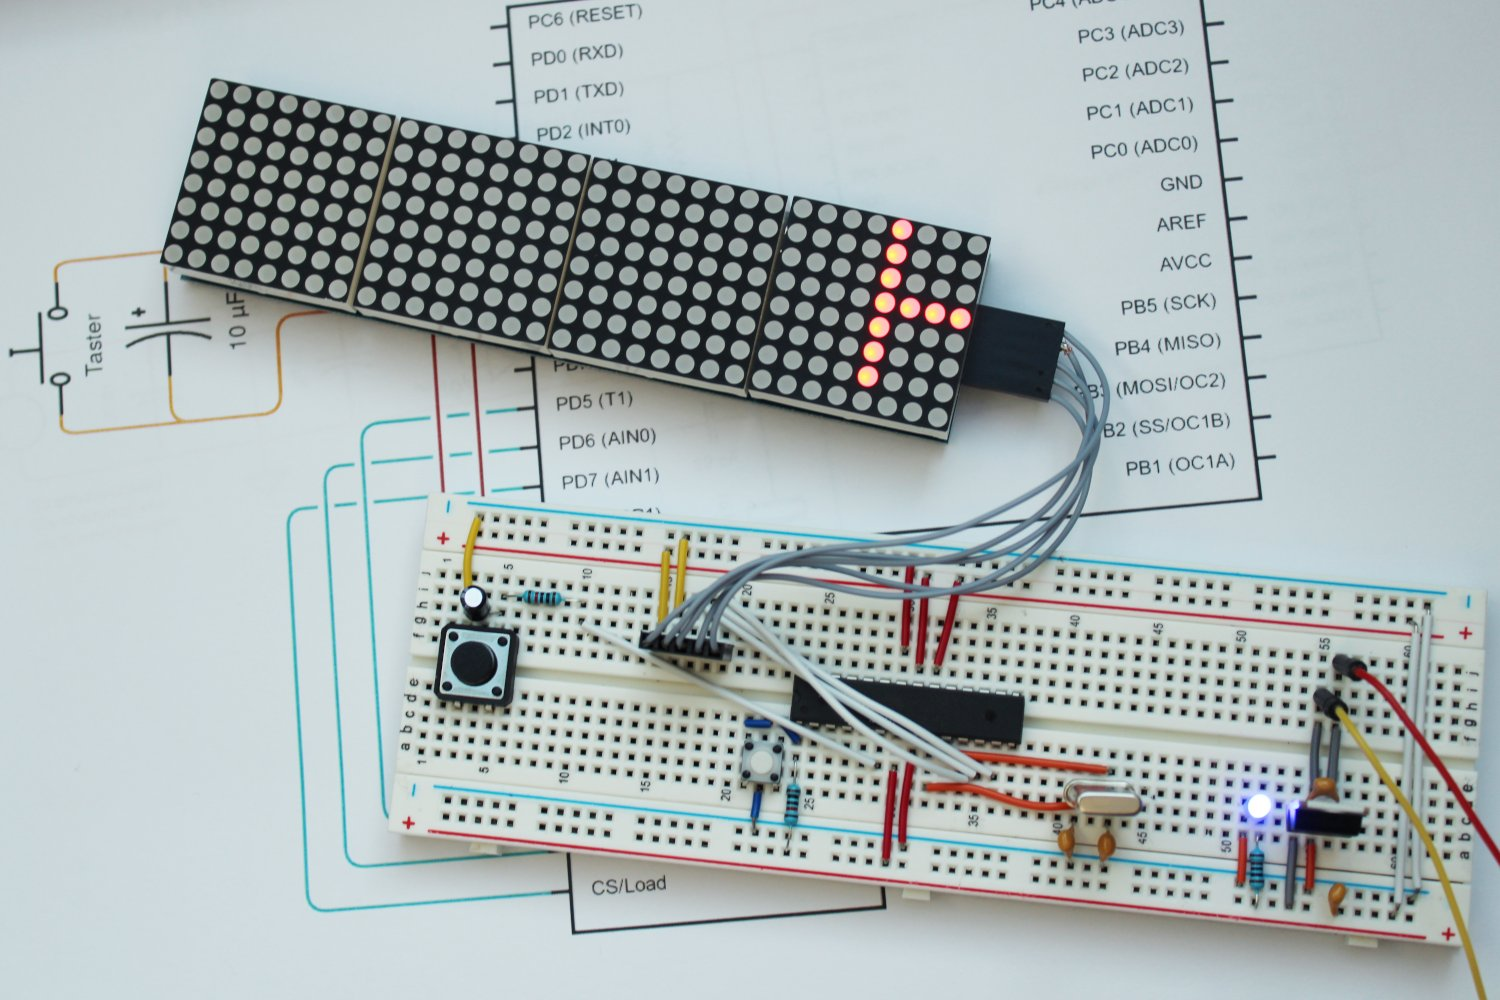
\includegraphics[width=\textwidth]{1-grundlagen/img/laufschrift_arduino2}
    \end{columns}
\end{frame}

{
\footnotesize

%%% Folie
\begin{frame}{Typischer Systemaufbau eingebetteter Systeme}
    \begin{columns}
        \column{\dimexpr\paperwidth}
        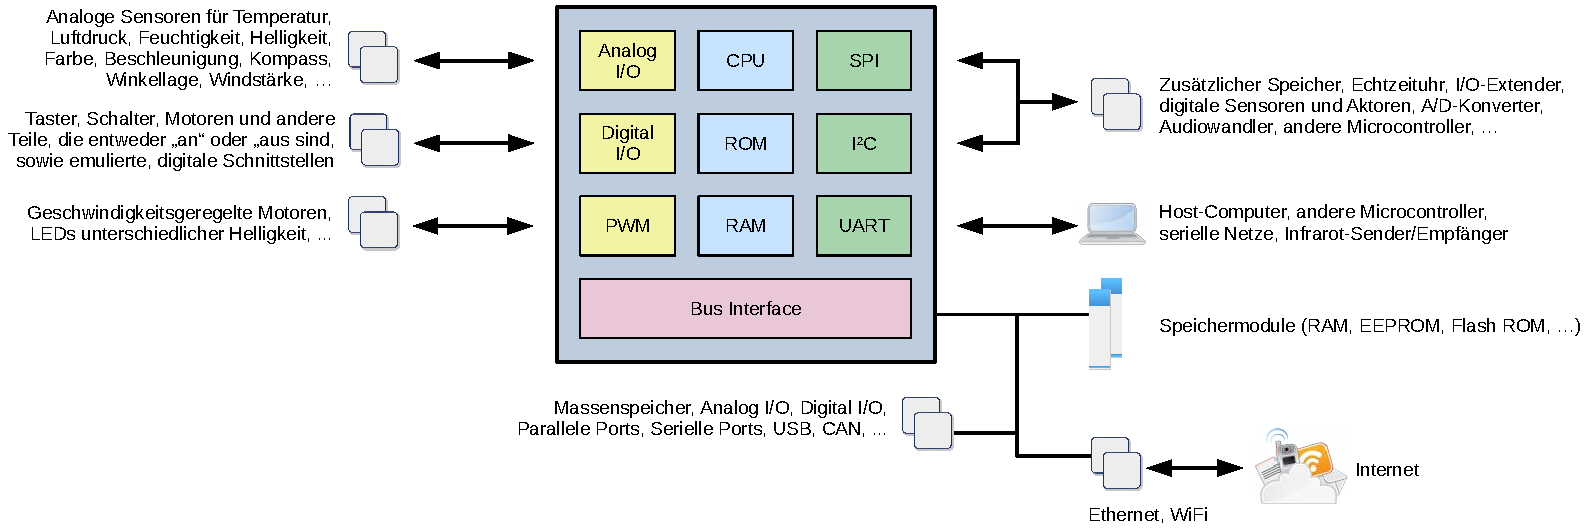
\includegraphics[width=\paperwidth]{1-grundlagen/img/mc_aufbau}
    \end{columns}

    \bigskip

    \begin{columns}
        \begin{column}[T]{.5\textwidth}
            \textbf{Durchschnittlicher Microcontroller}
            \begin{itemize}
                \item 16 MHz Taktgeschwindigkeit
                \item 8 Bit Wortbreite
                \item 32 kB Programmspeicher
                \item 2 kB Hauptspeicher
                \item 14 General Purpose I/Os
                \item Kein Betriebssystem
            \end{itemize}
        \end{column}
        \begin{column}[T]{.5\textwidth}
            \textbf{Durchschnittlicher System-on-a-Chip}
            \begin{itemize}
                \item $\geq$ 200 MHz Taktgeschwindigkeit
                \item $\geq$ 32 Bit Wortbreite
                \item $\geq$ 512 MB Flash ROM
                \item $\geq$ 16 MB Hauptspeicher
                \item $\geq$ 30 General Purpose I/Os
                \item Mit oder ohne Betriebssystem
            \end{itemize}
        \end{column}
    \end{columns}
\end{frame}
}

%%% Folie
{
    \setbeamertemplate{background canvas}{
        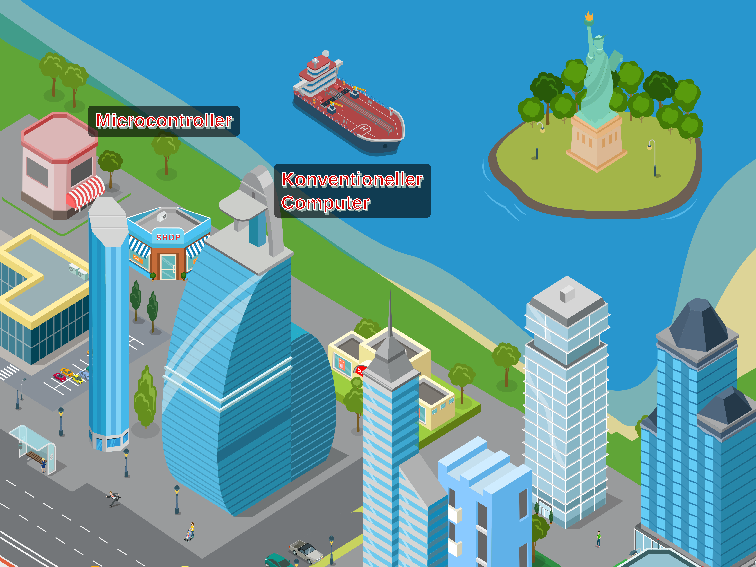
\includegraphics[height=\paperheight, width=\paperwidth]{1-grundlagen/img/software-abstraktion1}
    }

    \begin{frame}[plain]
        \transdissolve

        \only<beamer:2|handout:0>{
            \transdissolve

            \begin{tikzpicture}[remember picture,overlay]
                \node at (5.4cm,-0.97cm){
                    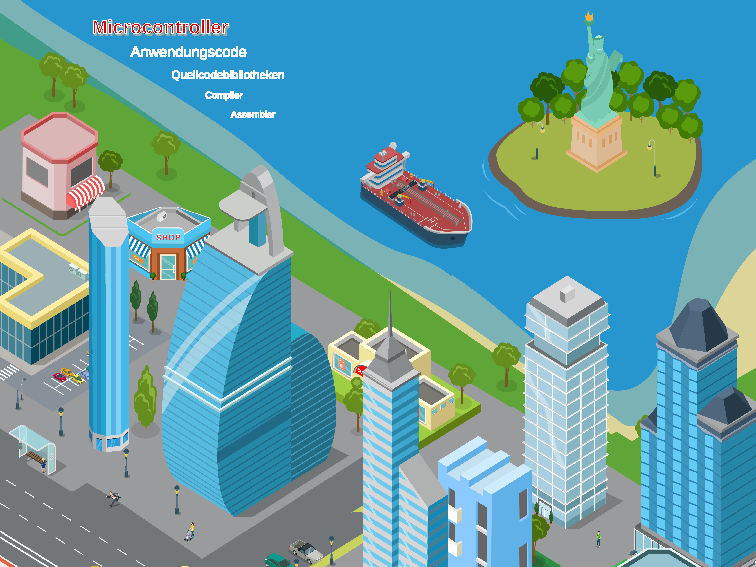
\includegraphics[height=\paperheight, width=\paperwidth]{1-grundlagen/img/software-abstraktion2}
                };
            \end{tikzpicture}
        }

        \only<beamer:3|handout:0>{
            \transdissolve

            \begin{tikzpicture}[remember picture,overlay]
                \node at (5.4cm,-0.97cm){
                    \includegraphics[height=\paperheight, width=\paperwidth]{1-grundlagen/img/software-abstraktion3}
                };
            \end{tikzpicture}
        }
    \end{frame}
}{
    \setbeamertemplate{background canvas}{
        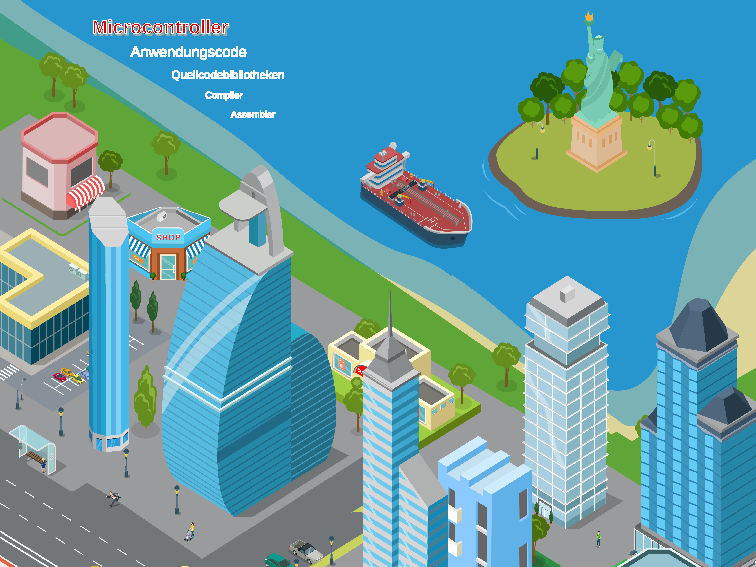
\includegraphics[height=\paperheight, width=\paperwidth]{1-grundlagen/img/software-abstraktion2}
    }

    \begin{frame}<handout>[plain]
        \transdissolve
    \end{frame}
}{
    \setbeamertemplate{background canvas}{
        \includegraphics[height=\paperheight, width=\paperwidth]{1-grundlagen/img/software-abstraktion3}
    }

    \begin{frame}<handout>[plain]
        \transdissolve
    \end{frame}
}



%%% Folie
\begin{frame}{Softwareseitige Systemanforderungen}
    \begin{columns}
        \column[T]{.5\textwidth}
        \begin{itemize}
            \item<1-> Sparsamer Umgang mit besonders knappen Ressourcen
            \item<2-> Verwendung spezialisierter Hardwarekomponenten
            \item<3-> Störungsfreier Betrieb über sehr lange Zeiträume
            \item<4-> Firmware-Upgrade ,,over the air''
        \end{itemize}

        \column[T]{.5\textwidth}
        \begin{itemize}
            \item<5-> Vollständig deterministisches Systemverhalten
            \item<6-> Oftmals daher nur begrenztes Multi-Tasking
            \item<7-> Harte, weiche oder eventuelle Echtzeitanforderungen
            \item<8-> Ausschalten des Geräts ohne ,,Herunterfahren''
        \end{itemize}
    \end{columns}

    \uncover<9->{
        \parbox{\linewidth}{
            \bigskip
            Zur Erfüllung dieser Anforderungen kommen in der Regel angepasste und
            besonders schlanke, eingebettete Betriebssysteme zum Einsatz, falls
            überhaupt ein Betriebssystem vorhanden ist. Hierbei kann es sich entweder
            um speziell für diesen Zweck entwickelte Betriebssysteme wie FreeRTOS
            und ITRON oder um eine angepasste Variante größerer Betriebssysteme wie
            Linux handeln. Linux bietet sich aufgrund seiner Quelloffenheit und
            leichten Portierbarkeit besonders an und wird daher auch entsprechend
            oft genutzt.
        }
    }
\end{frame}
